% This is the MAIN DOCUMENT of the Thesis MSc TEMPLATE.
% The content for the Thesis MSc is to be written in separate documents
% located in the folder ./Chapters
%         Aknowledgments.tex
%         Abstract.tex
%         KeyWords.tex
%         Resumo.tex
%         PalavrasChave.tex
%         Acronyms.tex
%         Front_Cover.tex
%         Chapter_1.tex ....Chapter_2 .....
%         ApendixA.tex ... ApendixB.tex...
% -----------------------------------------------------------------------------
% The class "istulthesis" is based on the standard LaTeX 'report' class.
% It can be used for Instituto Superior Tecnico thesis, as it follows the 
% regulations published by the Scientific Council of IST.
% The class defines the document style. 
% IST requires the thesis to be written in Arial or similar. 
% Two arguments in '\documentclass' allow you to define the thesis font: 
% 'Helvetica' and 'AvantGarde', which transforms 
% the default LaTeX font into Helvetica or AvantGarde, respectively.
% #############################################################################
% The document is automatically set for english or portuguese by just selecting
% the MAIN LANGUAGE in file 'Thesis-MSc-Preamble_commands.tex' 
% #############################################################################
% Thesis-MSc
% Version 4, August 2022
% BY: Prof. Rui Santos Cruz, rui.s.cruz@tecnico.ulisboa.pt
% #############################################################################
% !TEX root = ./main.tex
% -----------------------------------------------------------------------------
%
%\documentclass[defaultstyle,10pt,Helvetica,oneside]{istulthesis}
\documentclass[defaultstyle,10pt,Helvetica,twoside,openright]{istulthesis}
%
% -----------------------------------------------------------------------------
% The Preamble document contains all the necessary Packages for typesetting
% Modify it to suit your needs
% -----------------------------------------------------------------------------
% #############################################################################
% Preamble for Thesis-MSc in English or Portuguese
% Required Packages and commands
% --> Please Choose the MAIN LANGUAGE for the Thesis in package BABEL (below)
% !TEX root = ./main.tex
% #############################################################################
% Thesis-MSc
% Version 4, August 2022
% BY: Prof. Rui Santos Cruz, rui.s.cruz@tecnico.ulisboa.pt
% #############################################################################
%
% -----------------------------------------------------------------------------
% PACKAGES ucs, utf8x, babel, iflang:
% -----------------------------------------------------------------------------
% The 'ucs' package provides support for using UTF-8 in LaTeX documents. 
% However in most situations it is not required.
\usepackage{ucs}
% The 'utf8' package contains support for using UTF-8 as input encoding. 
\usepackage[utf8]{inputenc}
\usepackage[T1]{fontenc}
% The 'babel' package may correct some hyphenation issues of LaTeX. 
% Select your MAIN LANGUAGE for the Thesis with the 'main=' option.
\usepackage[main=english,portuguese]{babel}
% The 'iflang' package is used to help determine the language being used. 
\usepackage{iflang}


% -----------------------------------------------------------------------------
% PACKAGE scrbase:
% -----------------------------------------------------------------------------
% The 'scrbase' package is used to help redefining document structure.
\usepackage{scrbase}
% -----------------------------------------------------------------------------
% PACKAGE mathtools, amsmath, amsthm, amssymb, amsfonts, nicefrac:
% -----------------------------------------------------------------------------
% These packages are typically required. 
% Among many other things they add the possibility to put symbols in bold
% by using \boldsymbol (not \mathbf); defines additional fonts and symbols;
% adds the \eqref command for citing equations.
\usepackage{mathtools, amsmath, amsthm, amssymb, amsfonts}
\usepackage{nicefrac}
%
% -----------------------------------------------------------------------------
% PACKAGE tikz:
% -----------------------------------------------------------------------------
% Tikz  for creating graphics programmatically.
\usepackage{tikz}
\usetikzlibrary{shapes.geometric, arrows, positioning}
% -----------------------------------------------------------------------------
% PACKAGES array, booktabs, multirow, colortbl, spreadtab:
% -----------------------------------------------------------------------------
% These packages are most usefull for advanced tables. 
% 'multirow' allows to join rows throuhg the command \multirow which works
% similarly with the command \multicolumn.
% The 'colortbl' package allows to color the table (foreground and background)
% The package 'booktabs' provide some additional commands to enhance
% the quality of tables
% The 'longtable' package is only required when tables extend beyond the length
% of one page, which typically does not happen and should be avoided
\usepackage{array}
\usepackage{booktabs}
\usepackage{multirow}
\usepackage{colortbl}
\usepackage{spreadtab}
\usepackage{longtable}
\usepackage{pdflscape}
\usepackage{float}
%
% -----------------------------------------------------------------------------
% PACKAGES graphicx, subfigure:
% -----------------------------------------------------------------------------
% The package 'graphicx' supports formats PNG and JPG.
% Package 'subfigure' allows to place figures within figures with own caption. 
% For each of the subfigures use the command \subfigure.
\usepackage{graphicx}
\usepackage[hang,small,bf,tight]{subfigure}
%
% -----------------------------------------------------------------------------
% PACKAGE caption:
% -----------------------------------------------------------------------------
% The 'caption' package offers customization of captions in floating 
% environments such figure and table
% \usepackage[hang,small,bf]{caption}
\usepackage[format=hang,labelfont=bf,font=small]{caption} 
% the following customization adds vertical space between caption and the table
\captionsetup[table]{skip=10pt}
%
% -----------------------------------------------------------------------------
% PACKAGE algorithmic, algorithm, algorithm2e:
% -----------------------------------------------------------------------------
% These packages are required if you need to describe an algorithm.
% The preference is for using 'algorithm2e'
%\usepackage{algorithmic}
%\usepackage[chapter]{algorithm}
% \usepackage[ruled,vlined,algochapter,norelsize,\languagename]{algorithm2e}
\usepackage{algorithm}
\usepackage{algpseudocode}
%
% -----------------------------------------------------------------------------
% PACKAGE listings
% -----------------------------------------------------------------------------
% These packages are required if you need to list code snippets.
\usepackage{listings}
% Nicely syntax highlighted m-code in LaTeX documents with stylefile mcode.sty
% http://www.mathworks.com/matlabcentral/fileexchange/8015-m-code-latex-package
\usepackage[numbered]{mcode}
%
% -----------------------------------------------------------------------------
% Re-define listings captions and titles based on language.
\newcaptionname{portuguese}{\lstlistingname}{Listagem} % Listings CAPTIONS
\newcaptionname{portuguese}{\lstlistlistingname}{Listagens} % LIST of LISTINGS
%
% -----------------------------------------------------------------------------
% PACKAGE csquotes
% -----------------------------------------------------------------------------
% Quotation helper package
\usepackage{csquotes}
%
% -----------------------------------------------------------------------------
% PACKAGE todonotes
% -----------------------------------------------------------------------------
% Create TODO Notes in text
% The notes can be made invisible by just using the 'disable' option:
\usepackage[textwidth=2cm, textsize=small]{todonotes}
%\usepackage[textwidth=2cm, textsize=small, disable]{todonotes}
\setlength{\marginparwidth}{2cm}
%
% -----------------------------------------------------------------------------
% PACKAGE changes
% -----------------------------------------------------------------------------
% Track changes in document (changes in pdf preview).
%% Use "final" option to make all tracking markups invisible.
%\usepackage[authormarkup=superscript,authormarkuptext=id,markup=underlined,ulem={ULforem,normalbf},final]{changes}
\usepackage[authormarkup=superscript,authormarkuptext=id,markup=underlined,ulem={ULforem,normalbf}]{changes}
% commands:
% \added[id=xx]{text}
% \deleted[id=xx]{text}
% \replaced[id=xx]{deleted text}{added text}
% -----------------------------------------------------------------------------
% PACKAGES xcolor, color
% -----------------------------------------------------------------------------
% These packages are required for list code snippets.
\usepackage{xcolor}
\usepackage{color}
% The following special color definitions are used in the IST Thesis
\definecolor{forestgreen}{RGB}{34,139,34}
\definecolor{orangered}{RGB}{239,134,64}
\definecolor{lightred}{rgb}{1,0.4,0.5}
\definecolor{orange}{rgb}{1,0.45,0.13}	
\definecolor{darkblue}{rgb}{0.0,0.0,0.6}
\definecolor{lightblue}{rgb}{0.1,0.57,0.7}
\definecolor{gray}{rgb}{0.4,0.4,0.4}
\definecolor{lightgray}{rgb}{0.95, 0.95, 0.95}
\definecolor{darkgray}{rgb}{0.4, 0.4, 0.4}
\definecolor{editorGray}{rgb}{0.95, 0.95, 0.95}
\definecolor{editorOcher}{rgb}{1, 0.5, 0} % #FF7F00 -> rgb(239, 169, 0)
\definecolor{chaptergrey}{rgb}{0.6,0.6,0.6}
\definecolor{editorGreen}{rgb}{0, 0.5, 0} % #007C00 -> rgb(0, 124, 0)
\definecolor{olive}{rgb}{0.17,0.59,0.20}
\definecolor{brown}{rgb}{0.69,0.31,0.31}
\definecolor{purple}{rgb}{0.38,0.18,0.81}
%
% -----------------------------------------------------------------------------
% PACKAGE setspace:
% ----------------------------------------------------------------------------
% Provides support for setting the spacing between lines in a document. 
% Package options include single spacing, one half spacing, and double spacing. 
% Alternatively the spacing can be changed as required with:
% \singlespacing, \onehalfspacing, and \doublespacing commands
\usepackage{setspace}
%
% -----------------------------------------------------------------------------
% PACKAGE paralist
% -----------------------------------------------------------------------------
% This package provides the 'inparaenum' environment for inline lists
\usepackage{paralist}
% usage:
% \begin{inparaenum}[(a)]
% \item bla
% \item bla, bla
% \end{inparaenum}
% -----------------------------------------------------------------------------
% PACKAGE cite:
% -----------------------------------------------------------------------------
% The 'cite' package will result in citation numbers being automatically
% sorted and properly "ranged". i.e.,
% [1], [2], [5]--[7], [9]
\usepackage{cite}
%
% -----------------------------------------------------------------------------
% PACKAGE acronym:
% -----------------------------------------------------------------------------
% The package 'acronym' garantees that all acronyms definitions are 
% given at the first usage. 
% IMPORTANT: do not use acronyms in titles/captions; otherwise the definition 
% will appear on the table of contents.
\usepackage[printonlyused]{acronym}
%
% -----------------------------------------------------------------------------
% PACKAGE hyperref
% -----------------------------------------------------------------------------
% Set links for references and citations in document
\usepackage{hyperref}
% pre-configuration of hyperref
\hypersetup{ colorlinks=true,
             citecolor=cyan,
             linkcolor=darkgray,
             urlcolor=teal,
             breaklinks=true,
             bookmarksnumbered=true,
             bookmarksopen=true,
}
%
% -----------------------------------------------------------------------------
% PACKAGE url:
% -----------------------------------------------------------------------------
% Provides better support for handling and breaking URLs.
\usepackage{url} 
%
% -----------------------------------------------------------------------------
% PACKAGE Cleveref:
% -----------------------------------------------------------------------------
% Clever Referencing of document parts
% use \Cref[], or \cref[] for referencing items (Figures, Tables, Algorythms, 
% Equations, Chapters, Sections, etc. No need to write the Name of the item. 
% Note: portuguese is supported through "brazilian" option
\usepackage[\IfLanguageName{english}{english}{brazilian}]{cleveref}
%
% -----------------------------------------------------------------------------
% PACKAGE enumitem:
% -----------------------------------------------------------------------------
%For enhanced enumeration of lists
%\usepackage{enumitem}
\usepackage[shortlabels]{enumitem}
\setlist[description]{leftmargin=\parindent,labelindent=\parindent,itemsep=1pt,parsep=0pt,topsep=0pt}
%
% -----------------------------------------------------------------------------
% PACKAGE glossaries-extra:
% -----------------------------------------------------------------------------
% Allows creating a list of terms with definitions for those terms
\usepackage[xindy,nopostdot]{glossaries}

% Special style to print trailing dots before locations list
\makeatletter
\newglossarystyle{mystyle}{%
  \setglossarystyle{altlist}%
  \renewenvironment{theglossary}{%
  \begin{description}[style=standard,labelindent=0pt,itemsep=5pt]%
  }%
  {\end{description}}
  \renewcommand*{\glossentry}[2]{%
    \item[\glsentryitem{##1}%
      \glstarget{##1}{\glossentryname{##1}}]%
      \mbox{}\par\nobreak\@afterheading
      \glossentrydesc{##1}\glspostdescription
      {\def\hfill{\hskip 25pt plus 3fill}\dotfill\mbox{ ##2}}%
  }%
  \renewcommand{\glsgroupskip}{}%
}
\makeatother
\setglossarystyle{mystyle}

\makeglossaries

\newglossaryentry{maths}
{
    name=mathematics,
    description={Mathematics is what mathematicians do}
}

\newglossaryentry{LaTeX}
{
    name=LaTeX,
    description={LaTeX It is a mark up language specially suited for scientific documents as it can correctly format documents with all the typographical rules}
}


\newglossaryentry{formula}
{
    name=formula,
    description={A mathematical expression}
}
% #############################################################################
% GLOBAL FORMATTING OF THE THESIS DOCUMENT before using FANCY stuff
% Load Titlepage definition
\usepackage{./cover-titlepage}

% Set paragraph counter to alphanumeric mode
% DO NOT CHANGE these lines, otherwise the document will not respect the Guide
\renewcommand{\theparagraph}{\Alph{paragraph}~--}
\hoffset 0in
\voffset 0in
\oddsidemargin 0 cm
\evensidemargin 0 cm
\marginparsep 0in
\topmargin -0.25cm
\textwidth 16 cm
\textheight 22.4 cm
\makeatletter
% package indentfirst says \let\@afterindentfalse\@afterindenttrue
% and we revert this modification, reinstating the original definitio
% of \@afterindentfalse
\def\@afterindentfalse{\let\if@afterindent\iffalse}
\makeatother
% -----------------------------------------------------------------------------
% PACKAGE fancyhdr:
% -----------------------------------------------------------------------------
% The fancyhdr macro package allows to customize page headers and footers.
\usepackage{fancyhdr}
\pagestyle{fancy}
\renewcommand{\chaptermark}[1]{\markboth{\thechapter.\ #1}{}}
\renewcommand{\sectionmark}[1]{\markright{\thesection\ #1}}
\fancyhf{}
%#########################################################
% Choose the positioning of the Page Number
% Only on the Center side [C]
\fancyfoot[C]{\bfseries\thepage}
% Only on the Right side [R]
%\fancyfoot[R]{\bfseries\thepage}
% In case of Double sided printing, numbers are printed on Left (even pages) and on Right (odd pages)
%\fancyfoot[LE,RO]{\bfseries\thepage}
%#########################################################
\renewcommand{\headrulewidth}{0.0pt}
\renewcommand{\footrulewidth}{0.0pt}
\addtolength{\headheight}{2pt} % make space for the rule

\fancypagestyle{plain}{%
   \renewcommand{\headrulewidth}{0pt} % and the line
   \renewcommand{\footrulewidth}{0pt}
}
\fancypagestyle{blank}{%
   \renewcommand{\headrulewidth}{0pt} % and the line
   \renewcommand{\footrulewidth}{0pt}
}
\fancypagestyle{abstract}{%
   \renewcommand{\headrulewidth}{0pt}
   \renewcommand{\footrulewidth}{0.0pt}
}
\fancypagestyle{document}{%
	\renewcommand{\headrulewidth}{0.5pt}
	\renewcommand{\footrulewidth}{0.5pt}
	\addtolength{\headheight}{2pt} % make space for the rule
}
\setcounter{secnumdepth} {5}
\setcounter{tocdepth} {5}
\renewcommand{\thesubsubsection}{\thesubsection.\Alph{subsubsection}}
\renewcommand{\subfigtopskip}{0.3 cm}
\renewcommand{\subfigbottomskip}{0.2 cm}
\renewcommand{\subfigcapskip}{0.3 cm}
\renewcommand{\subfigcapmargin}{0.2 cm}

\usepackage{etoc}
\newcommand{\chaptoc}{%
  \etocsettocstyle{\section*{Contents}}{}%
  \localtableofcontents
}

%
% -----------------------------------------------------------------------------
% PACKAGE minitoc:
% -----------------------------------------------------------------------------
% Package 'minitoc' creates a mini-table of contents (a “minitoc”) at 
% the beginning of each chapter of a document.
% This packages are required for the \fancychapter configuration
\usepackage{minitoc}
\setcounter{minitocdepth}{1}
\setlength{\mtcindent}{24pt}
\renewcommand{\mtcfont}{\small\rm}
\renewcommand{\mtcSfont}{\small\bf}
\renewcommand*{\kernafterminitoc}{\kern0.\baselineskip\kern0.ex}
\mtcselectlanguage{\languagename} 
% Now prepare the MINITOC
\def\boxedverbatim{%
  \def\verbatim@processline{%
    {\setbox0=\hbox{\the\verbatim@line}%
    \hsize=\wd0 \the\verbatim@line\par}}%
  \@minipagetrue%%%DPC%%%
  \@tempswatrue%%%DPC%%%
  \setbox0=\vbox\bgroup\vspace*{0.2cm}\footnotesize\verbatim
}
\def\endboxedverbatim{%
  \endverbatim
  \unskip\setbox0=\lastbox %%%DPC%%%
  \hspace*{0.2cm}
  \vspace*{-0.2cm}
  \egroup
  \fbox{\box0}% <<<=== change here for centering,...
}
% Now prepare the CHAPTER Number
\newcommand*{\chapnumfont}{%
%   \usefont{T1}{\@defaultcnfont}{b}{n}\fontsize{100}{130}\selectfont%
  \usefont{T1}{pbk}{b}{n}
  \fontsize{130}{100}
  \selectfont
  \color{chaptergrey}
}
\makeatletter
\def\@makechapterhead#1{%
  \vspace*{50\p@}%
  {\parindent \z@ \raggedright \normalfont
    {\chapnumfont\ifnum \c@secnumdepth >\m@ne
%         \huge\bfseries \@chapapp\space \thechapter
        \raggedleft\bfseries \thechapter
        \par\nobreak
        \vskip 20\p@
    \fi}
    \interlinepenalty\@M
    {\raggedleft\Huge \bfseries #1\par\nobreak}
    \vskip 40\p@
  }}
\makeatother
% Now put it all together as a command \fancychapter
\newcommand{\fancychapter}[1]{\chapter{#1}\minitoc\bigskip}

%
% #############################################################################
% ADDITIONAL COMMANDS AND CONFIGURATIONS
% #############################################################################
% This commmand allows to place horizontal lines with a custom width... 
% replaces the standard hline command
\newcommand{\hlinew}[1]{%
  \noalign{\ifnum0=`}\fi\hrule \@height #1 \futurelet
   \reserved@a\@xhline}
%   
% -----------------------------------------------------------------------------
% This command defines some marks... USEFUL FOR TABLES.
\def\Mark#1{\raisebox{0pt}[0pt][0pt]{\textsuperscript{\footnotesize\ensuremath{\ifcase#1\or *\or \dagger\or \ddagger\or%
    \mathsection\or \mathparagraph\or \|\or **\or \dagger\dagger%
    \or \ddagger\ddagger \else\textsuperscript{\expandafter\romannumeral#1}\fi}}}}
%


% -----------------------------------------------------------------------------
% The following configurations are used for LISTINGS of certain languages
\lstdefinestyle{XML} {
	language=XML,
	extendedchars=true, 
	breaklines=true,
	breakatwhitespace=true,
	emph={},
	emphstyle=\color{red},
	basicstyle=\small,
	xleftmargin=17pt,
	columns=fullflexible,
	commentstyle=\color{gray}\upshape,
	morestring=[b][\color{brown}]",
	morecomment=[s]{<?}{?>},
	morecomment=[s][\color{forestgreen}]{<!--}{-->},
	keywordstyle=\color{orangered},
	stringstyle=\ttfamily\color{black},
	% stringstyle=\ttfamily\color{black}\normalfont,
	tagstyle=\color{blue},
	% tagstyle=\color{darkblue}\bf,
	morekeywords={asn,action,addrType,abilityNAT,audioSampleRate,audiChannels,,bandwidth,bitmapSize,bitRate,connection,codecs,concurrentLinks,dependency,duration,frameRate,from,height,ip,id,lang,mimeType,onlineTime,peerMode,port,priority,peerProtocol,property,release,to,tier,type,transactionID,url,uploadBWlevel,version,width},
	otherkeywords={attribute,xmlns,schemaLocation,PresentationType,availabilityStartTime,availabilityEndTime,minimumUpdatePeriod,minBufferTime,UpdateTime},
}
% ----------------------------------------------------------------------------
\lstdefinelanguage{Assembler}{
	morecomment=[l];,
	keywords={ADD,ADDC,SUB,SUBB,CMP,MUL,DIV,MOD,NEG,AND,OR,NOT,XOR,TEST,BIT,SET,EI,EI0,EI1,EI2,EI3,SETC,EDMA,CLR,DI,DI0,DI1,DI2,DI3,CLRC,SHR,SHL,SHRA,SHLA,ROR,ROL,RORC,ROLC,MOV,MOVB,MOVBS,MOVP,MOVL,MOVH,SWAP,PUSH,POP,JZ,JNZ,JN,JNN,JP,JNP,JC,JNC,JV,JNV,JEQ,JNE,JLT,JLE,JGT,JGE,JA,JAE,JB,JBE,JMP,CALL,CALLF,RET,RETF,SWE,RFE,NOP},
	morekeywords={EQU,TABLE,WORD,STRING,PLACE},
} 
% ----------------------------------------------------------------------------
\lstdefinestyle{coloredASM}{
	language=Assembler,
	extendedchars=false,
	breaklines=true,
	tabsize=2,
	numberstyle=\tiny,
	numbers=left,
	breakatwhitespace=true,
	emph={},
	emphstyle=\color{red},
	fontadjust=true,
	basicstyle=\small\ttfamily,
	% basicstyle=\footnotesize\ttfamily,
	columns=fixed,
	xleftmargin=17pt,
	framexleftmargin=17pt,
	framexrightmargin=5pt,
	framexbottommargin=4pt,
	commentstyle=\color{forestgreen}\upshape,
	morestring=[b][\color{brown}]",
	keywordstyle=\color{darkblue},
	stringstyle=\ttfamily\color{black},
	literate={á}{{\'a}}1 {ã}{{\~a}}1 {â}{{\^a}}1 {é}{{\'e}}1 {É}{{\'E}}1 {ê}{{\^e}}1 {õ}{{\~o}}1 {ó}{{\'o}}1 {í}{{\'i}}1 {ç}{{\c{c}}}1 {Ç}{{\c{C}}}1,
}    
% ----------------------------------------------------------------------------
\lstdefinelanguage{CSS}{
	sensitive=true,
	morecomment=[l]{//},
	morecomment=[s]{/*}{*/},
	morestring=[b]',
	morestring=[b]",
	alsoletter={:},
	alsodigit={-},
	keywords={color,background-image:,margin,padding,font,weight,display,position,top,left,right,bottom,list,style,border,size,white,space,min,width, transition:, transform:, transition-property, transition-duration, transition-timing-function}
}
% ----------------------------------------------------------------------------
% JavaScript
\lstdefinelanguage{JavaScript}{
	morecomment=[s]{/*}{*/},
	morecomment=[l]//,
	morestring=[b]",
	morestring=[b]',
	morekeywords={typeof, new, true, false, catch, function, return, null, catch, switch, var, if, in, while, do, else, case, break}
}
% ----------------------------------------------------------------------------
\lstdefinelanguage{HTML5}{
	language=html,
	sensitive=true,	
	alsoletter={<>=-},	
	morecomment=[s]{<!-}{-->},
	tag=[s],
	otherkeywords={
	% General
	>,
	% Standard tags
	<!DOCTYPE,
	</html, <html, <head, <title, </title, <style, </style, <link, </head, <meta, />,
	% body
	</body, <body,
	% Divs
	</div, <div, </div>, 
	% Paragraphs
	</p, <p, </p>,
	% scripts
	</script, <script,
	% More tags...
	<canvas, /canvas>, <svg, <rect, <animateTransform, </rect>, </svg>, <video, <source, <iframe, </iframe>, </video>, <image, </image>, <header, </header, <article, </article},
	ndkeywords={
	% General
	=,
	% HTML attributes
	charset=, src=, id=, width=, height=, style=, type=, rel=, href=,
	% SVG attributes
	fill=, attributeName=, begin=, dur=, from=, to=, poster=, controls=, x=, y=, repeatCount=, xlink:href=,
	% properties
	margin:, padding:, background-image:, border:, top:, left:, position:, width:, height:, margin-top:, margin-bottom:, font-size:, line-height:,
	% CSS3 properties
	transform:, -moz-transform:, -webkit-transform:,
	animation:, -webkit-animation:,
	transition:,  transition-duration:, transition-property:, transition-timing-function:,
	}
}
% ----------------------------------------------------------------------------
\lstdefinestyle{htmlcssjs} {%
	% General design
	backgroundcolor=\color{editorGray},
		fontadjust=true,
	basicstyle=\small\ttfamily,   
	frame=b,
	% line-numbers
	xleftmargin={0.75cm},
	numbers=left,
	stepnumber=1,
	firstnumber=1,
	numberfirstline=true,	
	% Code design
	identifierstyle=\color{black},
	keywordstyle=\color{blue}\bfseries,
	ndkeywordstyle=\color{editorGreen}\bfseries,
	stringstyle=\color{editorOcher}\ttfamily,
	commentstyle=\color{brown}\ttfamily,
	% Code
	language=HTML5,
	alsolanguage=JavaScript,
	alsodigit={.:;},	
	tabsize=2,
	showtabs=false,
	showspaces=false,
	showstringspaces=false,
	extendedchars=true,
	breaklines=true,
	% German umlauts
	literate=%
	{Ö}{{\"O}}1
	{Ä}{{\"A}}1
	{Ü}{{\"U}}1
	{ß}{{\ss}}1
	{ü}{{\"u}}1
	{ä}{{\"a}}1
	{ö}{{\"o}}1
}
% ----------------------------------------------------------------------------
\lstdefinestyle{py} {%
	language=python,
	literate=%
	*{0}{{{\color{lightred}0}}}1
	{1}{{{\color{lightred}1}}}1
	{2}{{{\color{lightred}2}}}1
	{3}{{{\color{lightred}3}}}1
	{4}{{{\color{lightred}4}}}1
	{5}{{{\color{lightred}5}}}1
	{6}{{{\color{lightred}6}}}1
	{7}{{{\color{lightred}7}}}1
	{8}{{{\color{lightred}8}}}1
	{9}{{{\color{lightred}9}}}1,
	basicstyle=\small\ttfamily,
	numbers=left,
	% numberstyle=\tiny,
	% stepnumber=2,
	numbersep=5pt,
	tabsize=4,
	extendedchars=true,
	breaklines=true,
	keywordstyle=\color{blue}\bfseries,
	frame=b,
	commentstyle=\color{brown}\itshape,
	stringstyle=\color{editorOcher}\ttfamily,
	showspaces=false,
	showtabs=false,
	xleftmargin=17pt,
	framexleftmargin=17pt,
	framexrightmargin=5pt,
	framexbottommargin=4pt,
	backgroundcolor=\color{lightgray},
	showstringspaces=false,
}

% -----------------------------------------------------------------------------
% The official name of the course/degree. Automatic for MEIC. It depends on language
%
\IfLanguageName{english}
		{\degree{Computer Science and Engineering}}
		{\degree{Engenharia Informática e de Computadores}}

%
% #############################################################################
% #############################################################################
\begin{document}
%
% Add PDF bookmark 
\pdfbookmark[0]{Titlepage}{Title}
% #############################################################################
% DEFINE THE Front Cover Page of Thesis-MSc
% !TEX root = ./main.tex
% #############################################################################
% Thesis-MSc
% Version 4, August 2022
% BY: Prof. Rui Santos Cruz, rui.s.cruz@tecnico.ulisboa.pt
% #############################################################################
%
% REQUIRED LOGO:
% The university logo image: arguments correspond to {left}{top} position. 
% IST rules determine the position to be be 2cm from top, left page edge
\univlogo{20mm}{20mm}{./Images/IST_A_RGB_POS}
% OPTIONAL IMAGE:
% The thesis image: arguments are the start position in the page.
% You can change the image for your thesis, replacing the image name.
% If no image is desired, just comment the command
%\thesislogo{25mm}{50mm}{./Images/tecnico-lisboa}
%
% -----------------------------------------------------------------------------
% REQUIRED: Thesis TITLE
\title{This is the Title of the Thesis and it is a very Big Title covering More than One Line}
% OPTIONAL: Thesis SUBTITLE
%\subtitle{This is the Thesis Subtitle if Necessary}
%
% -----------------------------------------------------------------------------
% REQUIRED: Author
% Author full Name
\author{Diogo Alexandre Ferreira de Jesus}
%
%
% -----------------------------------------------------------------------------
% REQUIRED: The SUPERVISOR(s) - maximum of two
\supervisor{Luis Manuel Antunes Veiga}
% If no co-Supervisor comment the next line
\othersupervisor{Prof. Name of the Co-Supervisor}
%
% -----------------------------------------------------------------------------
% REQUIRED: Date of examination
% Insert the Date of the Thesis discussion (format is MONTH and YEAR)
\date{Month 20XX}
%
% -----------------------------------------------------------------------------
% The following command define the author colors for Tracking Changes in doc in case you use Tracking
% the Two letters identify each author
\definechangesauthor[color=forestgreen]{MN}
\definechangesauthor[color=blue]{JO}
\definechangesauthor[color=red]{PT}

% -----------------------------------------------------------------------------
% Select 'false' when delivering the draft version of the thesis.
% The committee members should not be printed for the draft version. 
% Select 'true' after the Examination Committee has accepted the thesis as final
\finalthesis{true}
%\finalthesis{false}
%
% -----------------------------------------------------------------------------
% The members of the Examination Committee
% Normally there is only the "vogalone"
% Uncomment the others if necessary
\chairperson{Prof. Name of the Chairperson}
\vogalone{Prof. Name of First Committee Member}
%\vogaltwo{Dr. Name of Second Committee Member}
%\vogalthree{Eng. Name of Third Committee Member}
%
% -----------------------------------------------------------------------------
% The second page should be white with the Copyright message.
% Print Titlepage (Cover)
\maketitle
\thispagestyle{empty} % the following page without header or footer
\cleardoublepage
%
% -----------------------------------------------------------------------------
% PAGE NUMBERING FOR INDEXING MATTER in ROMAN
\setcounter{page}{1} \pagenumbering{roman}
\baselineskip 18pt % line spacing: -12pt for single spacing
                   %               -18pt for 1 1/2 spacing
                   %               -24pt for double spacing
% -----------------------------------------------------------------------------
% THE ACKNOWLEGMENTS
\pdfbookmark[0]{Acknowledgments}{acknowledgments}
\begin{acknowledgments}
	% #############################################################################
% Agradecimentos / Acknowledgments
% !TEX root = ../main.tex
% #############################################################################

I would like to thank my parents for their friendship, encouragement and caring over all these years, for always being there for me through thick and thin and without whom this project would not be possible. I would also like to thank my grandparents, aunts, uncles and cousins for their understanding and support throughout all these years.

Quisque facilisis erat a dui. Nam malesuada ornare dolor. Cras gravida, diam sit amet rhoncus ornare, erat elit consectetuer erat, id egestas pede nibh eget odio. Proin tincidunt, velit vel porta elementum, magna diam molestie sapien, non aliquet massa pede eu diam. Aliquam iaculis. 

Fusce et ipsum et nulla tristique facilisis. Donec eget sem sit amet ligula viverra gravida. Etiam vehicula urna vel turpis. Suspendisse sagittis ante a urna. Morbi a est quis orci consequat rutrum. Nullam egestas feugiat felis. Integer adipiscing semper ligula. Nunc molestie, nisl sit amet cursus convallis, sapien lectus pretium metus, vitae pretium enim wisi id lectus. 

Donec vestibulum. Etiam vel nibh. Nulla facilisi. Mauris pharetra. Donec augue. Fusce ultrices, neque id dignissim ultrices, tellus mauris dictum elit, vel lacinia enim metus eu nunc.

I would also like to acknowledge my dissertation supervisors Prof. Some Name and Prof. Some Other Name for their insight, support and sharing of knowledge that has made this Thesis possible.

Last but not least, to all my friends and colleagues that helped me grow as a person and were always there for me during the good and bad times in my life. Thank you.

To each and every one of you -- Thank you.
\end{acknowledgments}
%
% -----------------------------------------------------------------------------
% THE ABSTRACT
\begin{abstract}
	% #############################################################################
% Abstract Text
% !TEX root = ../main.tex
% #############################################################################
% reset acronyms
\acresetall
% use \noindent in firts paragraph
\noindent Nulla facilisi. In vel sem. Morbi id urna in diam dignissim feugiat. Proin molestie tortor eu velit. Aliquam erat volutpat. Nullam ultrices, diam tempus vulputate egestas, eros pede varius leo, sed imperdiet lectus est ornare odio. Lorem ipsum dolor sit amet, consectetuer adipiscing elit. Proin consectetuer velit in dui. Phasellus wisi purus, interdum vitae, rutrum accumsan, viverra in, velit. Sed enim risus, congue non, tristique in, commodo eu, metus. Aenean tortor mi, imperdiet id, gravida eu, posuere eu, felis. Mauris sollicitudin, turpis in hendrerit sodales, lectus ipsum pellentesque ligula, sit amet scelerisque urna nibh ut arcu. Aliquam in lacus. Vestibulum ante ipsum primis in faucibus orci luctus et ultrices posuere cubilia Curae; Nulla placerat aliquam wisi. Mauris viverra odio. Quisque fermentum pulvinar odio. Proin posuere est vitae ligula. Etiam euismod. Cras a eros.
\end{abstract}
\begin{keywords}
	% #############################################################################
% English Keywords
% !TEX root = ../main.tex
% #############################################################################
% reset acronyms
\acresetall
% use \noindent in firts paragraph
\noindent Maecenas tempus dictum libero; Donec non tortor in arcu mollis feugiat;Cras rutrum pulvinar tellus.
\end{keywords}
\clearpage
\thispagestyle{empty}
%% If Printing on DOUBLE SIDED pages, the second page should be white.
%% Otherwise, comment the following command:
\cleardoublepage
%
% -----------------------------------------------------------------------------
% O RESUMO
\begin{resumo}
	% #############################################################################
% RESUMO em Português
% !TEX root = ../main.tex
% #############################################################################
% reset acronyms
\acresetall
% use \noindent in firts paragraph
\noindent Pellentesque habitant morbi tristique senectus et netus et malesuada fames ac turpis egestas. Vestibulum tortor quam, feugiat vitae, ultricies eget, tempor sit amet, ante. Donec eu libero sit amet quam egestas semper. Aenean ultricies mi vitae est. Mauris placerat eleifend leo. Quisque sit amet est et sapien ullamcorper pharetra. Vestibulum erat wisi, condimentum sed, commodo vitae, ornare sit amet, wisi. Aenean fermentum, elit eget tincidunt condimentum, eros ipsum rutrum orci, sagittis tempus lacus enim ac dui. Donec non enim in turpis pulvinar facilisis. Ut felis. Aliquam aliquet, est a ullamcorper condimentum, tellus nulla fringilla elit, a iaculis nulla turpis sed wisi. Fusce volutpat. Etiam sodales ante id nunc. Proin ornare dignissim lacus. Nunc porttitor nunc a sem. Sed sollicitudin velit eu magna. Aliquam erat volutpat. Vivamus ornare est non wisi. Proin vel quam. Vivamus egestas. Nunc tempor diam vehicula mauris. Nullam sapien eros, facilisis vel, eleifend non, auctor dapibus, pede.
\end{resumo}
\begin{palavraschave}
	% #############################################################################
% Portuguese Keywords
% !TEX root = ../main.tex
% #############################################################################
% reset acronyms
\acresetall
% use \noindent in firts paragraph
\noindent Cloud Computing; Serverless; FaaS; Serverless Workflows; Serverless DAGs; Metadata; Workflow Prediction
\end{palavraschave}
\clearpage
\thispagestyle{empty}
%% If Printing on DOUBLE SIDED pages, the second page should be white.
%% Otherwise, comment the following command:
\cleardoublepage
%
% -----------------------------------------------------------------------------
% This is required for the Fancy Chapters with minitoc
\dominitoc
\dominilof
\dominilot
% -----------------------------------------------------------------------------
% Lists of Contents
\renewcommand{\baselinestretch}{1}
\pdfbookmark[0]{Contents}{toc}
\tableofcontents
% If Printing on DOUBLE SIDED pages, the second page should be white.
% Otherwise, comment the following command:
\cleardoublepage
% reposition baseline
\renewcommand{\baselinestretch}{1.5}
% -----------------------------------------------------------------------------
% List of Figures
\pdfbookmark[1]{List of Figures}{lof}
\listoffigures
%\cleardoublepage
% -----------------------------------------------------------------------------
\begingroup 
    % \let\clearpage\relax
    % \let\cleardoublepage\relax
    % \let\cleardoublepage\relax
% List of Tables
\pdfbookmark[1]{List of Tables}{lot}
\listoftables
% If Printing on DOUBLE SIDED pages, the second page should be white.
% Otherwise, comment the following command:
%\let\cleardoublepage\relax
%\cleardoublepage
% -----------------------------------------------------------------------------
% List of Algorithms
% If not used, comments the lines!
% Requires packages algorithmic, algorithm
\pdfbookmark[1]{List of Algorithms}{loa}
\listofalgorithms
% If Printing on DOUBLE SIDED pages, the second page should be white.
\endgroup
% Otherwise, comment the following command:
%\cleardoublepage
% -----------------------------------------------------------------------------
% Listings
% If not used, comments the lines!
% Requires packages listings
\pdfbookmark[1]{Listings}{lol}
\lstlistoflistings
%\cleardoublepage
% -----------------------------------------------------------------------------
% % List of acronyms
\pdfbookmark[1]{Acronyms}{loac}
\chapter*{\tlangAcronyms}
% #############################################################################
% This is the ACRONYMS Definition
% !TEX root = ../main.tex
% #############################################################################
% Do not forget to reorder Alphabetically the ACRONYMS !!!
% If there are special cases for Plural form see example hereunder
\begin{acronym}[H.264/SVC]
	% \acro{DAG}{Directed Acyclic Graph}
	% \acro{FaaS}{Function-as-a-Service}
	% \acro{AAC}{Advanced Audio Coding}
	% \acro{ADTS}{Audio Data Transport Stream}
	% \acro{API}{Application Program Interface}
	% \acro{AS}{Application Server}
	% \acro{AV}{Audio-Visual}
	% \acro{AVC}{Advanced Video Coding}
	% \acro{BMFF}{Base Media File Format}
	% \acro{CC}{Cloud Computing}
	% \acro{CDN}{Content Distribution Network}
	% \acro{CPU}{Central Processing Unit}
	% \acro{DASH}{Dynamic Adaptive Streaming over HTTP}
	% \acro{DVD}{Digital Versatile Disk}	
	% \acro{ES}{Elementary Stream}
	% \acro{ftyp}{File Type}
	% \acro{FLV}{Flash Video}
	% \acro{GPRS}{General Packet Radio Service}
	% \acro{GSM}{Global System for Mobile Communications}
	% \acro{H.264/AVC}{Advanced Video Coding}
	% \acro{H.264/SVC}{Scalable Video Coding}
	% \acro{HD}{High Definition}
	% \acro{HDTV}{High Definition Television}
	% \acro{HLS}{HTTP Live Streaming}
	% \acro{HTTP}{Hypertext Transfer Protocol}
	% \acro{IaaS}{Infrastructure as a Service}
	% \acro{IETF}{Internet Engineering Task Force}
	% \acro{IGMP}{Internet Group Management Protocol}
	% \acro{IIS}{Internet Information Services}
	% \acro{IMS}{IP Multimedia Subsystem}
	% \acro{IP}{Internet Protocol}
	% \acro{IPTV}{IP Television}
	% \acro{ISP}{Internet Service Provider}
	% \acro{IT}{Information Technology}
	% \acro{JSVM}{Joint Scalable Video Model}
	% \acro{LAN}{Local Area Network}
	% \acro{LTE}{Long Term Evolution}
	% \acro{MDC}{Multiple Description Coding}
	% \acro{MIME}{Multipurpose Internet Mail Extension}
	% \acro{MPD}{Media Presentation Description}
	% \acro{MPEG}{Moving Picture Expert Group}
	% \acro{NAL}{Network Abstraction Layer}
	% \acro{NAT}{Network Address Translation}	
	% \acro{OS}{Operating System}
	% \acro{OSMF}{Open Source Media Framework}
	% \acro{P2P}{Peer-to-Peer}
	% \acro{PaaS}{Platform as a Service}
	% \acro{PES}{Packetized Elementary Streams}
	% \acro{QoE}{Quality Of Experience}
	% \acro{QoS}{Quality Of Service}
	% \acro{QP}{Quantization Parameter}
	% % ----------------------------------------
	% % this Acronym has a special plural version
	% \acro{RM}{Regenerative Medicine}
    % \acrodefplural{RM}{Regenerative Medicines}
    % % ----------------------------------------
	% \acro{RTCP}{RTP Control Protocol}
	% \acro{RTMP}{Real Time Messaging Protocol}
	% \acro{RTP}{Real-time Transport Protocol}
	% \acro{RTSP}{Real Time Streaming Protocol}
	% \acro{SaaS}{Software as a Service}
	% \acro{SD}{Standard Definition}
	% \acro{SEI}{Supplemental Enhancement Information}
	% \acro{SIP}{Selective Inter-layer Prediction}
	% \acro{SMS}{Short Message Service}
	% \acro{SNR}{Signal-to-Noise Ratio}
	% \acro{SVC}{Scalable Video Coding}
	% \acro{TCP}{Transport Control Protocol}
	% \acro{TS}{Transport Stream}
	% \acro{TTL}{Time-to-Live}
	% \acro{UDP}{User Datagram Protocol}
	% \acro{UI}{User Interface}
	% \acro{UMTS}{Universal Mobile Telecommunication System}
	% \acro{URL}{Uniform Resource Locator}
	% \acro{VCEG}{Video Content Expert Group}
	% \acro{VCL}{Video Coding Layer}
	% \acro{VoD}{Video On Demand}
	% \acro{WAN}{Wide Area Nework}
	% \acro{WLAN}{Wireless Local Area Network}
	% \acro{WMA}{Windows Media Audio}
	% \acro{WWAN}{Wireless Wide Area Network}		
	% \acro{XML}{Extensible Markup Language}
	% \acro{DQId}{Direct Quality ID}
	% \acro{DTD}{Document Type Definition}
	% \acro{IST}{Instituto Superior Tecnico}
	% \acro{EDGE}{Enhanced Data Rates for GSM Evolution}
	% \acro{SNS}{Social networking service}
\end{acronym}
% If Printing on DOUBLE SIDED pages, the second page should be white.
\clearpage
% -----------------------------------------------------------------------------
% Glossary
% Comment if not used
\pdfbookmark[1]{Glossary}{glo}
\printglossary[]
% Otherwise, comment the following command:
\cleardoublepage
% -----------------------------------------------------------------------------
% PAGE NUMBERING FOR DOCUMENT MATTER in ARABIC
% Pages number is starting with arabic style. Until here were on roman mode
\setcounter{page}{1} \pagenumbering{arabic}
\baselineskip 18pt
% -----------------------------------------------------------------------------
% This a suggestion for the Content of the Document
% Add more Chapters by duplicating a Chapter Block, pointing to the file
%Chapter 1
\acresetall
% #############################################################################
% This is Chapter 1
% !TEX root = ../main.tex
% #############################################################################
% Change the Name of the Chapter i the following line
\chapter{Introduction}
\chaptoc
% The following line allows to ref this chapter
\label{chap:intro}


Function-as-a-Service (FaaS) represents a serverless cloud computing paradigm that simplifies application deployment by abstracting away infrastructure management. It provides automatic, elastic scalability—potentially without limit—along with a fine-grained, pay-per-use pricing model. This has led to its widespread adoption for event-driven systems, microservices, and web services on platforms like AWS Lambda\footnote{\label{fn:aws-lambda}https://aws.amazon.com/pt/lambda/}, Azure Functions\footnote{\label{fn:azure-funcs}https://azure.microsoft.com/en-us/products/functions}, and Google Cloud Functions\footnote{\label{fn:google-cloud-functions}https://cloud.google.com/functions}. These applications typically benefit the most from FaaS because they are lightweight, stateless, and characterized by highly variable or unpredictable workloads, allowing them to leverage serverless platforms' on-demand scalability and cost-efficiency.

This paradigm is also increasingly used to execute complex scientific and data processing workflows, such as the Cybershake~\cite{cybershake_workflow} seismic hazard analysis or Montage~\cite{montage_astronomy}, an astronomy image mosaicking workflow. These applications are structured as workflows—formally represented as Directed Acyclic Graphs (DAGs) of interdependent tasks. However, efficiently executing these complex workflows on serverless platforms remains a significant challenge. 

Despite their advantages, serverless platforms present several limitations that complicate the execution of complex workflows. Since these platforms allow scaling down to zero resources to save costs, they can also introduce unpredictable latency, known as \textit{cold starts}~\cite{cold_starts_surey}, particularly for short-lived functions, affecting overall workflow performance. The lack of \textit{direct inter-function communication}~\cite{serverless_computing_drawbacks_survey_rw1} means that tasks often have to rely on external services, such as message brokers or databases to exchange intermediate data, which can increase overhead and reduce efficiency. Interoperability between platforms is further limited by the use of platform-specific workflow definition languages, which restricts the portability of workflows across different serverless environments. Additionally, while statelessness simplifies scaling and management, it can introduce overhead and complexity for applications that require continuity or coordination across multiple function invocations. Finally, developers have limited control over the underlying infrastructure, restricting the ability to optimize resource usage or tune performance for specific workloads.

Several solutions have emerged to address the limitations of serverless platforms. Stateful functions (e.g., AWS Step Functions\footnote{\label{fn:aws-step-functions}https://aws.amazon.com/pt/step-functions/}, Azure Durable Functions\footnote{\label{fn:azure-durable-functions}https://learn.microsoft.com/en-us/azure/azure-functions/durable/durable-functions-overview?tabs=in-process\%2Cnodejs-v3\%2Cv1-model\&pivots=csharp}, and Google Cloud Workflows\footnote{\label{fn:google-cloud-workflows}https://cloud.google.com/workflows}) expand the range of applications that can run on serverless platforms by maintaining state across multiple function invocations, coordinating complex workflows, and providing built-in fault tolerance. Other approaches tackle limitations at the runtime level, proposing extensions to FaaS platforms (e.g., Faa\$T~\cite{faast_caching}, Palette~\cite{palette_load_balancing}, Lambdata~\cite{lambdata_intents}) or entirely new serverless architectures (e.g., Apache OpenWhisk~\cite{open_whisk}). Finally, some workflow-focused solutions (e.g., WUKONG~\cite{wukong_2}, Unum~\cite{unum_decentralized_orchestrator}, DEWEv3~\cite{dewe_v3}) employ scheduling strategies and workflow-level optimizations to enhance efficiency, primarily by improving data locality to bring computation closer to the data and minimize reliance on external services.

These workflow-focused approaches, however, often use uniform resources for workers and rely on “one-step scheduling,” making decisions based solely on the immediate workflow stage without considering the broader context or the downstream effects of their decisions. This combination of homogeneous worker configurations and limited scheduling foresight can lead to inefficient use of resources when tasks have diverse computational or memory requirements. Furthermore, the heuristic-based approaches used by other solutions can be inefficient in certain scenarios, as they lack mechanisms to adapt worker resource allocations to the specific needs of individual tasks. Moreover, we found no prior work that leverages metadata or historical metrics to inform scheduling decisions across an entire serverless workflow.  

This limitation motivates the central research question of this work: if we have knowledge of the computation steps, collect sufficient metrics on their behavior, and understand how they are composed to form the full workflow, can we leverage this information to make smarter scheduling decisions that minimize makespan and maximize resource efficiency in a FaaS environment?  

To answer this research question, we propose a decentralized serverless workflow execution engine that leverages historical metadata from previous workflow runs to generate informed task allocation plans, which are then executed by FaaS workers in a choreographed manner, without needing a central scheduler. By relying on such planning, our approach aims to minimize the usage of external cloud storage services, which are often employed by similar solutions for intermediate data exchange and synchronization, while also avoiding the inefficiencies of homogeneous worker resource allocations.

The main contributions of this work are as follows:
\begin{itemize}
    \item Analysis of the serverless workflow orchestration research landscape;
    \item Propose a decentralized serverless workflow execution engine that overcomes the "one-step scheduling" and uniform-resource limitations of existing workflow-focused solutions by leveraging historical metadata to generate informed execution plans;
    \item Demonstrate how incorporating historical execution data can improve task allocation, reduce reliance on external cloud storage services, and enhance overall workflow efficiency on FaaS platforms.
\end{itemize}

% #############################################################################
\section{Problem/Motivation}
% see intro of paper and pic (if needed)

% #############################################################################
\section{Gaps in prior work}
% see intro of paper

% #############################################################################
\section{Proposed Solution}
% see intro of paper

% #############################################################################
\section{Document Organization}

% If Printing on DOUBLE SIDED pages, the second page should be white.
% Otherwise, comment the following command:
\cleardoublepage
%Chapter 3
% #############################################################################
% This is Chapter 3
% !TEX root = ../main.tex
% #############################################################################
% Change the Name of the Chapter i the following line
\chapter{Related Work}
\chaptoc
\label{chap:rw}
\bigskip

In this section, we explore the serverless computing landscape, starting by exposing the architecture of a typical serverless computing platform, referencing the use cases for this new cloud computing model, and presenting both commercial and open-source offerings. We also delve into workflows, showing how they can be represented, how they are run and managed, and contrasting traditional frameworks for workflow management with more recent solutions that explore cloud technologies, including serverless. Then, we write about three extension proposals to the current serverless platforms design, aiming to improve data locality. We finish this section by presenting relevant workflow orchestrators and schedulers (serverful, serverless, and hybrid) for executing tasks, highlighting their advantages but also some of their limitations and inefficiencies.

% #############################################################################
\section{Serverless Computing}

Traditionally, cloud applications have been deployed on virtual machines, such as Amazon EC2~\footnote{\url{https://aws.amazon.com/pt/ec2/}}, which provide full control over the operating system and runtime environment. This model allows predictable performance, flexible resource allocation, direct communication via local network interfaces between VMs, and the ability to run long-lived services, but it comes with significant operational overhead: developers must manage provisioning (which can take several minutes), scaling, patching, and fault tolerance. 

Serverless computing addresses these challenges by abstracting away infrastructure management, enabling developers to focus solely on application logic. At the storage and database layer, serverless databases and object stores automatically scale with demand and charge based on actual usage. At the application level, \textbf{Backend-as-a-Service} (BaaS) platforms offer ready-to-use components like authentication and messaging. Finally, at the compute layer, \textbf{Function-as-a-Service} (FaaS) provides the most flexible and fine-grained model, allowing developers to deploy individual functions that execute on demand in response to events. In this document, we focus specifically on FaaS, as it is the model most relevant to our work.

The Function-as-a-Service (FaaS) model is now offered by major cloud providers, including Amazon (Lambda\cite{aws_lambda}), Google (Cloud Run Functions\cite{google_cloud_run_functions}), Microsoft (Azure Functions\cite{azure_functions}), and Cloudflare (Workers~\cite{cloudflare_workers}). In addition to these commercial offerings, several open-source runtimes such as OpenWhisk\cite{open_whisk}, OpenFaaS\cite{openfaas}, and Knative\cite{knative} provide developers with alternatives for deploying FaaS in self-managed or hybrid environments.

\subsection{Advantages}
Recent industry reports~\footnote{\url{https://www.grandviewresearch.com/industry-analysis/serverless-computing-market-report}} show that serverless computing has seen rapid adoption over the last few years. For example, in 2024 the global serverless computing market was estimated at USD 24.51 billion, and it is projected to more than double to USD 52.13 billion by 2030, with a compound annual growth rate (CAGR) of about 14.1\%. Function-as-a-Service (FaaS) constitutes the majority service model, representing over 60\% of serverless market share in 2024. This rapid growth highlights the increasing appeal of serverless architectures, which can be attributed to the following key benefits:

\begin{itemize}
    \item{\textbf{Operational Simplicity} means that developers are abstracted away from the underlying infrastructure management, without worrying about server maintenance, scaling, or provisioning. This enables faster development and deployment cycles;}
    \item{\textbf{Scalability} means the FaaS runtime handles increasing workloads by automatically provisioning additional computational capacity as demand grows, ensuring that applications remain responsive and performant. This makes the FaaS model ideal for applications with \textit{highly variable} or \textit{unpredictable} usage patterns, where we don't know \textit{how many} or \textit{when} requests will arrive;}
    \item{\textbf{Pay-per-use}: FaaS provides a pricing model where users are only charged for the resources used during the actual execution time over the memory used by their functions, rather than for pre-allocated resources (as in Infrastructure-as-a-Service).}
\end{itemize}

Given these advantages, the serverless model is particularly attractive for applications with \textit{highly variable} or \textit{unpredictable} workloads, such as web services, event-driven pipelines, and real-time data processing. It also suits applications that benefit from rapid iteration and deployment, including microservices, and APIs, where minimizing operational overhead is crucial. Furthermore, serverless can be advantageous in cost-sensitive contexts, where pay-per-use pricing reduces expenses for workloads that do not require continuous execution.

These benefits make serverless computing attractive not only for simple, event-driven applications but also for more complex workflows. Serverless workflows are a composition of multiple computational tasks that are chained together to execute applications by orchestrating individual serverless functions into a coordinated sequence. Some workflows have been successfully experimented with on FaaS. Notable examples include ExCamera~\cite{excamera}, a highly parallel video encoding system; Montage~\cite{montage_astronomy}, an astronomical image mosaic generator; and CyberShake~\cite{cybershake_workflow}, a seismic hazard modeling framework.

\subsection{Limitations}
% limitations and when do they show (for which type of apps)
While these advantages make serverless computing highly appealing for a wide range of applications, the model is not without its limitations. As adoption has grown, both practitioners and researchers have identified several technical and architectural challenges that hinder its broader applicability and performance. A number of studies have systematically analyzed these issues, among which Li et al.~\cite{serverless_computing_survey_rw1} provides a comprehensive overview of the benefits, challenges, and open research opportunities in the serverless landscape. The challenges mentioned include:

\begin{itemize}
    \item \textbf{Startup Latencies}: It's the time it takes for a function to start executing user code. Cold starts (explained further) can be critical, especially for functions with short execution times;
    \item \textbf{Isolation}: In serverless, multiple users share the same computational resources (often the same Kernel). This makes it crucial to properly isolate execution environments of multiple users;
    \item \textbf{Scheduling Policies}: Traditional cloud computing policies were not designed to operate in dynamic and ephemeral environments, such as FaaS's;
    \item \textbf{Resource Management}: Particularly storage and networking, needs to be optimized (by service providers) to handle the low latency and scalability requirements of serverless computing. The lack of direct inter-function networking is an example of a limitation that narrows down the variety of applications that can currently run on FaaS, as some may not support the overhead of using intermediaries (external storage) for data exchange;
    \item \textbf{Fault-Tolerance}: Cloud platforms impose restrictions on developers by encouraging the development of \textit{idempotent functions}. This makes it easier for providers to implement fault-tolerance by retrying failed function executions.
\end{itemize}

Hellerstein et al. \cite{serverless_computing_drawbacks_survey_rw1} portrays FaaS as a \textit{"Data-Shipping Architecture"}, where data is intensively moved to code, through external storage services like databases, bucket storage or queues, to circumvent the limitation of inter-function direct communication. This can greatly degrade performance, while also incurring extra costs.

These limitations notably impact workflows—complex applications composed of multiple functions orchestrated into a Directed Acyclic Graph (DAG), where each function's output serves as input for subsequent functions. Such workflows are prevalent in scientific computing, data processing, and machine learning pipelines. 

\subsection{Research Efforts}

To overcome some of the inherent limitations of traditional Function-as-a-Service (FaaS) platforms, several research initiatives have proposed architectural innovations aimed at improving performance, scalability, and orchestration. Apache OpenWhisk~\cite{open_whisk} adopts a fully event-driven, trigger-based architecture, in which functions are invoked automatically in response to events, allowing for more responsive execution and efficient resource utilization. Its design supports complex workflows and fine-grained control over function composition, making it suitable for latency-sensitive and distributed applications. 

Building on similar principles, TriggerFlow~\cite{triggerflow} extends the trigger-based approach by implementing an \textit{event-condition-action} paradigm, enabling efficient orchestration of complex workflows such as state machines and DAGs. This allows high-volume event processing, dynamic scaling, and improved fault tolerance, making it well-suited for long-running scientific and data-intensive workflows. 

Another notable platform, OpenFaaS~\cite{openfaas}, fights \textit{vendor lock-in} by emphasizing simplicity and portability, allowing developers to deploy serverless functions on a wide range of infrastructures while maintaining an event-driven execution model. Collectively, these platforms show how architectural innovations—particularly in event handling and workflow orchestration—can mitigate many of the performance and scalability limitations found in conventional FaaS systems.

%%%%%%
While solutions such as OpenWhisk and TriggerFlow propose completely novel serverless architectures, others such as Palette Load Balancing~\cite{palette_load_balancing}, Faa\$T~\cite{faast_caching}, Pocket~\cite{pocket}, Pheromone~\cite{pheromone}, and Lambdata~\cite{lambdata_intents} propose extending either the FaaS runtime or the workflow definition language to address one of the most pressing limitation of the serverless paradigm: data management inefficiencies.

Palette~\cite{palette_load_balancing} is a FaaS runtime extension that improves data locality by introducing the concept of \textbf{``colors``} as \textit{locality hints}. These colors are parameters attached to function invocations, enabling the invoker to express the desired affinity between invocations without directly managing instances. Palette then uses these hints to route invocations with the same color to the same instance \textit{if possible}, allowing for data produced by one invocation to be readily available to subsequent invocations, reducing the need for expensive data transfers, as it would be required in a typical FaaS runtime. This extra control that Palette provides can be used by workflow schedulers, which have insights on the data dependencies between tasks, to try co-locating tasks which share data dependencies, for example, leading to greater performance while also reducing resource utilization.

Faa\$T (Function-as-a-Service Transparent Auto-scaling Cache)~\cite{faast_caching} tackles the same issue as Palette, locality, but does so on the data level, by adding a \textbf{transparent caching layer} into the FaaS runtime. Each application is assigned an in-memory \textit{cachelet} that stores frequently accessed data, enabling subsequent invocations to reuse it without resorting to remote storage. Cachelets cooperate as a distributed cache using \textit{consistent hashing} to share objects across instances, while pre-warming and auto-scaling mechanisms adapt the cache to workload demands. Unlike Palette, which requires user-provided hints, Faa\$T operates automatically, preserving the simplicity of the serverless model, hence the "transparent" in its name.

Similarly, Lambdata~\cite{lambdata_intents} improves data locality by relying on explicit \textbf{data intents} provided by the developer. Functions declare which objects they will read and write, allowing the controller to co-locate invocations that share data dependencies on the same worker and reuse a local cache. This reduces remote storage accesses and data transfer overheads. Compared to Palette's flexible color hints, Lambdata's data intents are more precise but place stricter requirements on developers, while contrasting with Faa\$T's fully automated and distributed approach. Contrasting with Palette, Lambdata requires less effort from the developer, but at the cost of reduced flexibility.

% #############################################################################
\section{Workflows}
As stated before, workflows represent systematic methodologies for organizing and executing computational processes, providing a structured approach to designing, managing, and reproducing generic computations. Workflows have proven to be useful for many different use cases, from application payments and order processing, to data analytics pipelines that move and transform large datasets, to scientific computing and simulations where complex experiments are broken into manageable steps. 

\subsection{Workflow Definition Languages}
% workflow definition languages (see pic.pdf)
At their conceptual core, most workflows can be represented as directed acyclic graphs (DAGs), which model computational processes by depicting tasks as nodes and their dependencies as edges connecting them. As an example of a typical web application workflow, consider an online payment process. When a user makes a purchase, the workflow can be represented as a DAG, where each task corresponds to a step in the transaction process. The first task may involve verifying the user's credentials, followed by tasks such as checking product availability, processing payment, and confirming the order. Each of these tasks \textit{depends on} the successful completion of the previous step, with dependencies that ensure the correct order of operations. For instance, payment processing cannot proceed without confirming the product availability, and order confirmation only occurs once payment has been processed. This simple DAG structure ensures that each task is executed in sequence, while also \textit{enabling parallel execution} where possible, such as checking product availability and verifying payment simultaneously.

Despite the existence of other ways to express workflows, due to the simplicity of writing and interpreting DAGs, most systems and libraries use this representation. For instance, Apache Airflow\cite{apache_airflow} uses DAGs to define and schedule workflows defined in Python. Similarly, Dask\cite{dask_python}, a Python parallel computing library, also utilizes DAGs to represent task dependencies, enabling the parallel execution of tasks across clusters. DAGMan (Directed Acyclic Graph Manager)\cite{dagman} is a way HTCondor\cite{htcondor} (distributed computing job manager) users can organize independent jobs into workflows, also in the form of DAGs.

However, there are more flexible alternatives to define workflows. YAWL (Yet Another Workflow Language)\cite{yawl} is a \textit{workflow language} that provides a highly expressive framework for workflow management, capable of supporting a wider range of workflow patterns. YAWL uses Petri networks\cite{petri_nets} instead of DAGs to model workflows. This allows YAWL to handle more complex control-flow structures, such as loops, parallelism, and advanced synchronization patterns, offering greater flexibility and power in defining and managing intricate workflows.

While using more capable and flexible workflow languages, such as \textit{YAWL} (Yet Another Workflow Language) allows the representation of more complex workflow patterns, most of the tools used for defining and running scientific workflows, like \textit{Apache Airflow}, \textit{Dask}, and HTCondor's DAGMan use the Directed Acyclic Graph format. This is because DAGs effectively model the majority of scientific workflows, which typically involve non-cyclic dependencies, making them simpler to compose, deploy, understand, debug, and visualize.

\subsection{Traditional Workflow Scheduling}
Going from a workflow definition to actual execution involves several key stages: provisioning resources to match computational demands, uploading code, dependencies, and data to ensure a consistent execution environment, scheduling tasks efficiently to optimize cost and performance, monitoring execution for performance and fault detection, and finally deprovisioning resources once the workflow completes. Traditional scheduling approaches from Grid and Cloud computing assume centralized control, which does not fully align with the ephemeral, stateless nature of serverless computing. Serverless platforms, however, can simplify many of these stages by automating resource scaling, data staging, fault handling, monitoring, and teardown, reducing operational overhead while adapting execution to dynamic workloads.

To alleviate some of the developers and researchers' pain points during these steps while scheduling workflows on more traditional \textit{Infrastructure as a Service} (IaaS) platforms, several data processing and workflow scheduling frameworks have emerged. Among the platforms for \textbf{data processing pipelines} are Apache Spark\cite{apache_spark}, Apache Flink\cite{apache_flink}, and Apache Hadoop\cite{apache_hadoop}, which focus on processing and analyzing large datasets efficiently through parallel and distributed computing. On the \textbf{workflow scheduling and orchestration} side, traditional platforms include Apache Oozie\cite{apache_oozie} and HTCondor\cite{htcondor}, which manage the execution and coordination of complex sequences of tasks, ensuring that dependencies are handled and resources are allocated effectively. These frameworks help streamline both the data processing and the management of workflows.

Apache Hadoop provided a foundation for large-scale data processing when it introduced the MapReduce~\cite{mapreduce} paradigm, supported by HDFS and YARN~\cite{yarn} for reliable storage and resource management. Apache Spark provides a flexible distributed model with rich libraries for analytics and efficient task dependency management, while Apache Flink specializes in real-time stream processing with low latency and robust state handling. In terms of workflow orchestration, Apache Oozie specializes in coordinating Hadoop-based tasks, whereas HTCondor targets high-throughput scientific workflows, efficiently managing complex dependencies. 

Similarly, Dask~\cite{dask_python} and its distributed scheduler (Dask Distributed~\cite{dask_python_distributed}) extend the familiar Python ecosystem to large-scale data and compute workloads, enabling parallel execution of array, dataframe, and machine learning operations across clusters, with a lightweight task graph scheduler that supports both batch and interactive computation. Together, these frameworks illustrate the range of solutions available for executing and coordinating workflows on top of the IaaS model, spanning batch and streaming data as well as data-centric and scientific computing environments.

While these frameworks address many critical aspects of resource provisioning, code and dependency management, and workflow monitoring, they rely on the \textit{Infrastructure as a Service} (IaaS) model. While offering significant flexibility and control over the computing environment, \textit{IaaS} comes with notable drawbacks as mentioned previously. A major challenge of IaaS platforms is the complexity of \textit{managing and provisioning} virtual machines, storage, and network resources, which requires expertise and incurs significant overhead. Users must also handle scaling, load balancing, and fault tolerance manually, often leading to inefficiencies. Predicting resource requirements is difficult, often resulting in \textit{over-} or \textit{under-provisioning}, and the typical hourly billing model can further increase costs, particularly for short workflows that run for only a few minutes.

As highlighted previously, the \textit{serverless} paradigm excels in scenarios where automatic scaling and cost-efficiency are essential, while also providing a much easier set-up process for developers by abstracting away the underlying infrastructure and only requiring the user to follow a few coding rules and minor configuration. Despite its current inefficiencies, the serverless model shows great potential for efficiently running the same types of data processing pipelines and workflows as those handled by the frameworks previously mentioned. Next, we will explore some of the most relevant solutions for scheduling serverless workflows.

\subsection{Modern Workflow Scheduling}

The limitations of IaaS-based frameworks, such as those mentioned previously, have led to a new generation of workflow orchestrators designed for flexibility, usability, and ease of deployment. Unlike earlier systems bound to static clusters and rigid DSLs, modern platforms embrace Python APIs, containerization~\footnote{\url{https://aws.amazon.com/what-is/containerization/}}, and cloud-native~\footnote{\url{https://aws.amazon.com/what-is/cloud-native/}} principles. Tools such as Prefect~\cite{prefect}, Dagster~\cite{dagster}, and Airflow~\cite{apache_airflow} prioritize developer productivity and observability, while Argo Workflows~\cite{argo_workflows} leverages Kubernetes~\cite{kubernetes} as its native execution environment. Another interesting project is Apache Beam, a cloud-native \textit{unified programming model} for batch and streaming data pipelines designed to be executed across multiple backends, with some of the most popular implementations being Google Cloud Dataflow~\cite{google_dataflow}. These solutions mark a shift from infrastructure management toward higher-level abstractions that integrate seamlessly with cloud platforms and services.

\subsubsection{Stateful Serverless Functions}

While modern orchestrators such as Argo, Prefect, Dagster, and Airflow provide powerful abstractions for coordinating workflows across diverse environments, they can be unnecessarily complex for developers who already rely on stateless serverless functions within a single cloud provider. In such cases, what is often required is not a general-purpose orchestration framework but a lightweight mechanism to compose stateless functions into more complex workflows, supporting coordination patterns such as \textit{fan-out}, \textit{fan-in}, and conditional branching. To address this gap, cloud providers have introduced \textit{stateful serverless functions}, which augment the stateless Function-as-a-Service (FaaS) model with durable state management and execution control.

A \textbf{stateful serverless function} represents a workflow orchestration paradigm in which an external coordination layer manages the execution and state of multiple stateless function invocations. These orchestrators track workflow progress, preserve context across invocations, and handle retries, error propagation, and branching logic. A common mechanism across these platforms is the use of \textit{snapshotting} or durable state persistence: the engine periodically records workflow state so that execution can be paused and later resumed without requiring all individual functions to remain active. By combining snapshotting with techniques such as event sourcing, persistent queues, and transactional state management, stateful orchestrators enable long-running workflows that can scale across distributed environments while remaining fault tolerant and cost efficient.

Prominent examples include AWS Step Functions~\cite{aws_step_functions}, Google Cloud Workflows~\cite{google_cloud_workflows}, Azure Durable Functions~\cite{azure_durable_functions}, and Cloudflare Workflows~\cite{cloudflare_workflows}. Despite differences in design and integration, they share the goal of simplifying complex coordination atop serverless platforms. AWS Step Functions offers JSON- or YAML-based state machines using the Amazon States Language (ASL)\footnote{\url{https://docs.aws.amazon.com/step-functions/latest/dg/concepts-amazon-states-language.html}}, enabling workflows that may last up to one year. Google Cloud Workflows provides YAML- or JSON-based definitions with a maximum duration of 60 minutes per execution, tightly integrated with Google Cloud services such as BigQuery and Cloud Run. Azure Durable Functions follows a code-centric approach in which developers write an \textit{"orchestrator function"} in languages such as C\#, JavaScript, or Python, with workflow durations of up to 30 days. Finally, Cloudflare Workflows emphasizes lightweight, edge-native~\footnote{\url{https://www.cloudflare.com/learning/serverless/glossary/what-is-edge-computing/}} orchestration, optimized for event-driven scenarios at the edge.

Together, these services extend the applicability of serverless beyond short-lived, stateless tasks, enabling complex approval processes, data pipelines, machine learning training, and financial transaction workflows that require state persistence and long execution durations. At the same time, they shift the responsibility of orchestration away from developers, who would otherwise need to implement custom, serverful coordination layers. 

The tradeoff, however, is strong vendor lock-in, since each provider enforces its own workflow representation and tight integration with its ecosystem, making portability and hybrid-cloud adoption more challenging. Furthermore, the user is billed for the orchestration service on top of the individual function executions, which can increase costs for long-running or highly parallel workflows compared to managing orchestration independently. In addition, the orchestrator can make suboptimal scheduling decisions, such as inefficient task placement or resource allocation, over which the user has little or no control, potentially impacting performance and cost efficiency.

\subsection{Serverless Workflow Scheduling}
% mention that it is implemented by rewriting parts of Dask Distributed!!
Having discussed commercial stateful serverless functions and their advantages and limitations, we now turn to research-oriented approaches for orchestrating workflows in stateless serverless environments. Unlike managed offerings, some of these systems explore innovative scheduling strategies and trade-offs that are particularly relevant for our work.

\subsubsection{Workflow Scheduling Approaches}

Workflow scheduling/orchestration in serverless environments can generally be categorized into three approaches:

\begin{itemize}
\item \textbf{Centralized scheduling:} In this approach, a single scheduler maintains a global view of the entire workflow, including task dependencies, resource availability, and execution progress. This allows the scheduler to make fine-grained decisions about task placement, load balancing, and prioritization, often optimizing for latency or resource utilization. However, the centralized model can become a bottleneck as workflow size and concurrency increase, introducing single points of failure. It also requires the scheduler to handle high-throughput metadata and state management, which can be challenging in highly dynamic serverless environments.

\item \textbf{Queue-based or message-driven scheduling:} Here, tasks are decoupled from execution using queues or message-passing systems. Producers submit tasks to a queue, and workers pull tasks asynchronously when they become idle. This design improves elasticity, as workers can scale independently of the workflow controller, and naturally provides fault tolerance—failed tasks can be retried by re-queuing. While it removes the single bottleneck of a centralized scheduler, queue-based systems may have less optimal global scheduling decisions, and additional logic may be needed to enforce task ordering or dependency constraints.

\item \textbf{Decentralized and Choreographed scheduling:} In this model, the responsibility for orchestration is distributed across the worker nodes rather than concentrated in a central entity. Each node independently manages task execution, coordinates with peers, and propagates state updates as necessary. This approach eliminates the need for dedicated scheduler infrastructure, mitigates bottlenecks, and enables faster scaling to thousands of concurrent functions. However, this model introduces greater complexity in ensuring fault tolerance and consistent state propagation across distributed, ephemeral environments. Ensuring that tasks execute \textit{exactly once} becomes particularly challenging, requiring stronger coordination and consensus mechanisms. To address these issues, algorithms such as Paxos~\cite{paxos}, Raft~\cite{raft}, or coordination services like ZooKeeper~\cite{zookeeper} can be employed, along with localized snapshots or lightweight distributed state stores, to maintain workflow coherence and reliability without relying on centralized scheduling. Most existing solutions, however, assume that tasks are \textit{idempotent}, so that repeated execution does not produce unintended side effects, simplifying failure recovery and avoiding the need for strict exactly-once guarantees.

\subsubsection{Relevant Workflow Schedulers}

To illustrate the spectrum of serverless workflow scheduling strategies, we now discuss representative systems that embody each approach and inspired our work. DEWE v3~\cite{dewe_v3} demonstrates a hybrid (IaaS and FaaS) queue-based model, where tasks are distributed through dedicated queues depending on their expected execution time. PyWren~\cite{pywren} exemplifies a more centralized scheduling paradigm, in which the user or submission machine maintains control over task execution while workers simply carry out assigned functions. Finally, Unum~\cite{unum_decentralized_orchestrator} and WUKONG~\cite{wukong_2} showcase decentralized choreographed orchestration, distributing workflow logic across workers to achieve high scalability and reduced reliance on central schedulers. Examining these systems provides concrete examples of the trade-offs and optimizations inherent to each scheduling strategy.

\paragraph{DEWE v3}
DEWE v3~\cite{dewe_v3} introduces an innovative hybrid approach to serverless workflow orchestration that combines the best aspects of both serverless and serverful computing models. This hybrid workflow execution engine intelligently distributes tasks based on their characteristics: \textit{short tasks} are run on FaaS workers while \textit{longer tasks} run on virtual machines. The system employs a queue-based job distribution mechanism where jobs expected to complete within FaaS limits are published to a common job queue for serverless execution, while long-running jobs are directed to a separate queue for local, serverful execution on dedicated servers. 

Jobs that fail to execute on FaaS workers, for being longer than expected and exceeding execution limits imposed by the platform, are redirected to the serverful queue. This dual-execution model enables DEWE to accommodate workflows with diverse resource consumption patterns. This system proves particularly effective for scientific workflows, such as Montage~\cite{montage_astronomy}, where task durations and resource requirements vary significantly. However, this hybrid approach introduces specific trade-offs. Latency-sensitive workflows may be slowed by job queuing overhead. In addition, hybrid deployments often lead to resource underutilization, as serverful workers may sit idle when most tasks are executed on FaaS. Finally, the centralized workflow manager can become a scalability bottleneck when handling many short tasks.

\paragraph{PyWren}
PyWren~\cite{pywren}, representing one of the pioneering pure serverless approaches, demonstrates the potential and limitations of leveraging unmodified serverless infrastructure for distributed computation. Built atop AWS Lambda, PyWren focuses on executing arbitrary Python functions as stateless serverless functions with minimal user management overhead, automatically handling function execution, dependencies, S3 bucket storage for serialized code and intermediate data. The system is ideal for \textit{embarrassingly parallel} workloads, also known as \textit{"bag-of-tasks"} scenarios, with many independent, parallel tasks such as simple data transformations, scientific simulations, parallel model training, and large-scale media processing. 
While PyWren's serverless orchestration model provides excellent scalability and removes the burden of infrastructure management, its simplicity limits its applicability. It is not well-suited for workflows with complex dependency structures or those that require sharing large intermediate results through object storage. Moreover, latency-sensitive applications are disadvantaged by function cold starts, since PyWren does not include mechanisms to mitigate their impact.

\paragraph{Unum}
Unum~\cite{unum_decentralized_orchestrator} takes a radically different approach from the two previous solutions by decentralizing orchestration logic entirely, eliminating the need for a standalone orchestrator service. This application-level serverless workflow orchestration system embeds orchestration logic directly into a library that wraps user-defined FaaS functions, leveraging an external scalable consistent data store for coordination during fan-ins and execution correctness. Unum introduces an Intermediate Representation (IR) to capture information about workflow progression (nearby tasks) and relies only on minimal, common serverless APIs (function invocation and basic data store operations) available across cloud platforms. This design choice provides exceptional portability and cost-effectiveness, as it can run on unmodified serverless infrastructure.

Unum also can and compile workflows defined in languages from providers like AWS Step Functions and Google Cloud Workflows into its IR format. However, Unum's generic approach comes with trade-offs: it currently supports only statically defined control structures and cannot express workflows where the next step is determined dynamically at runtime, and it lacks data locality optimizations since it cannot force related tasks to execute on the same worker, with each function instance executing only its specific task before triggering the next function.

\subsubsection{WUKONG}
WUKONG~\cite{wukong_2} represents the most sophisticated approach among these solutions, designed as a \textit{decentralized choreographed locality-enhanced} serverless workflow engine. Built on top of Dask's programming model and DAG generation capabilities~\cite{wukong_2}, WUKONG reimagines the execution layer to address the limitations of traditional serverful models like Dask Distributed while maximizing the advantages of serverless computing. The system focuses on improving scale-out speed and enhancing data locality to minimize large object movement. WUKONG's architecture is divided into static components (operating before workflow execution) and dynamic components (operating during execution). The static scheduler includes a \textbf{DAG Generator} that leverages Dask's library to convert Python code into DAGs, a \textbf{Schedule Generator} that creates \texttt{n} static schedules for \texttt{n} root/leaf nodes (each containing every reachable task in a depth-first search starting at that node), \textbf{Initial Task Executor Invokers} that launches the first Lambda instances for each root task, and a \textbf{Subscriber Process} on the client that waits for and downloads final results.

After receiving the initial schedules, FaaS workers (referenced to as \textit{AWS Lambda Executors}) drive workflow execution. Workers execute tasks until they encounter a \textit{fan-out}, at which point they transfer data to intermediate storage, execute 1 of the \texttt{N} fan-out tasks and invoke \textit{N - 1} \textit{new} executors for the other tasks. Then, when they find a \textit{fan-in}, the group of executors that reach the common fan-in node cooperate using a \textit{dynamic scheduling} model to select only one executor to proceed. This coordination is managed through a shared \textbf{dependency counter} in a Key-Value Store (KVS). Each involved executor \textit{atomically} updates this counter; the one whose update satisfies the final input dependency for the fan-in task will execute that task and continue along its static schedule. The other executors transfer their intermediate data to storage, and then stop their execution, decreasing the workflow parallelism.

Besides dynamic scheduling, WUKONG employs data locality optimization techniques designed to avoid moving large data objects; \textbf{Task Clustering for Fan-Out Operations} allows executors to continue executing downstream tasks when a fan-out task produces large outputs, becoming the executor of multiple fan-out targets rather than just executing 1 and invoking \texttt{N - 1} new executors; \textbf{Task Clustering for Fan-In Operations} enables executors to recheck dependencies after uploading large objects to storage, potentially executing fan-in tasks themselves if dependencies are satisfied during the upload process, potentially avoiding large downloads; \textbf{Delayed I/O} allows executors to hold off on writing large intermediate results to external storage until it is absolutely necessary. Instead of immediately storing data when some downstream tasks are not yet ready, the executor first runs any tasks that can proceed and then checks again if the remaining ones have become ready. If they have, the executor can execute them directly using the data already in memory, avoiding both the write and a later read from storage. Only when no further progress is possible are the results finally written out. This can reduce unnecessary data transfers.

These optimizations, combined with WUKONG's decentralized scheduling approach, significantly enhance performance compared to both \textbf{Dask Distributed} and \textbf{PyWren} by minimizing data transfer overhead and eliminating central scheduler bottlenecks. However, WUKONG shares the limitation of supporting only statically defined control structures, requiring workflow DAGs to be known ahead-of-time, similarly to our proposed solution. Additionally, its optimization heuristics can lead to inefficiencies in certain scenarios: \textit{Delayed I/O} may increase makespan and storage usage if dependencies aren't met after retries; fan-in conflicts where multiple tasks produce large objects can result in resource waste depending on upload timing; and fan-out scenarios with small inputs may not justify the overhead of invoking multiple executors as it can make subsequent fan-in's more expensive. Furthermore, WUKONG assumes a homogeneous execution environment, where all workers provide identical resources (e.g., each task is allocated 2 CPU cores and 512 MB of memory), which prevents tailoring resources to tasks with different computational or memory demands.

While WUKONG represents a significant advance in serverless workflow orchestration through its decentralization, its scheduling and optimizations remain limited. The system bases decisions only on the next stage of the workflow (i.e., one-to-one, fan-in, or fan-out transitions). We refer to this as \textit{one-step scheduling}, since it relies solely on information about the next step. Crucially, WUKONG does not exploit the global knowledge of the workflow structure, even though the entire workflow structure is known before execution begins. Also, its optimizations rely on heuristic-based strategies that can lead to suboptimal performance when workflow behavior deviates from expected patterns.

\end{itemize}

% #############################################################################
\section{Discussion/Analysis}
The existing body of related work highlights a clear progression in workflow orchestration strategies, moving from traditional cluster-based frameworks to cloud-native platforms and finally to serverless execution engines. Cluster-based systems such as Hadoop, Spark, Flink, and Dask emphasize fine-grained control, strong data locality, and predictable performance, but they incur significant operational overhead, limited elasticity, and often require technical expertise to deploy and manage. Commercial cloud-native platforms like AWS Step Functions and Azure Durable Functions simplify deployment and management by abstracting state handling and orchestration, but they typically incur additional costs and are bound to vendor-specific ecosystems. Runtime extensions such as Palette, Faa\$T, and Lambdata tackle the core inefficiencies of serverless platforms by enhancing data locality and reducing communication overhead.

Serverless workflow engines like PyWren, Unum, and WUKONG represent the most direct attempts to build high-performance workflow execution on unmodified FaaS infrastructure. While PyWren demonstrates the feasibility of large-scale embarrassingly parallel workloads, it struggles with complex workflows. Unum advances decentralization by embedding orchestration logic directly into functions, achieving portability and cost efficiency, but it remains limited in its support for dynamic control structures and lacks optimizations for data locality. WUKONG achieves major improvements through decentralization and data-aware heuristics such as \textit{Task Clustering} and \textit{Delayed I/O}, delivering great scalability and cost efficiency. Taken together, these systems provided the most direct inspiration for our work, while also highlighting key open challenges that our approach seeks to address.
% If Printing on DOUBLE SIDED pages, the second page should be white.
% Otherwise, comment the following command:
\cleardoublepage
%
%Chapter 4
% #############################################################################
% This is Chapter 4
% !TEX root = ../main.tex
% #############################################################################
% Change the Name of the Chapter i the following line
\chapter{Architecture}
\chaptoc
% The following line allows to ref this chapter
\label{chap:arch}

% #############################################################################
\section{Workflow Definition Language}
% see "paper.pdf"

% #############################################################################
\section{Overview}
% see "paper.pdf"

% #############################################################################
\section{Metadata Management}
% storage, type of data stored

% #############################################################################
\section{Static Workflow Planning}

\subsection{Simulation Layer}
% Metrics collected, how predictions are done/cached to be faster

\subsection{Planners}
% show some pseudocode

\begin{algorithm}
    \caption{Worker Assignment Algorithm}
    \label{alg:worker_assignment}
    \small
    \begin{algorithmic}[1]
    \Require $nodes$, $predictions$, $base\_rc$, $SLA$, $MAX\_CLUSTERING$
    \State $assigned \gets \emptyset$
    
    \Comment{nodes are topologically sorted}
    \ForAll{$n \in nodes$}
        \If{$n \in assigned$}
            \State \textbf{continue}
        \EndIf
        
        \If{$n.upstream = \emptyset$} \Comment{root nodes}
            \State $roots \gets \{r \in nodes \mid r.upstream = \emptyset \land r \notin assigned\}$
            \State \Call{AssignGroup}{$\textit{null}$, $roots$}
        \ElsIf{$|n.upstream| = 1$} \Comment{1$\to$1 or 1$\to$N}
            \State $u \gets n.upstream[0]$
            \If{$|u.downstream| = 1$}
                \State \Call{AssignWorker}{$[n]$, $u.worker$} \Comment{reuse worker}
            \Else \Comment{1$\to$N}
                \State $fanout \gets \{d \in u.downstream \mid d \notin assigned\}$
                \State \Call{AssignGroup}{$u.worker$, $fanout$}
            \EndIf
        \Else \Comment{N$\to$1}
            \State $outputs \gets \{u.worker: predictions.output\_size(u) \mid u \in n.upstream\}$
            \State $best \gets \arg\max_{w \in outputs} outputs[w]$
            \State \Call{AssignWorker}{$[n]$, $best$}
        \EndIf
    \EndFor
    
    \Statex
    
    \Function{AssignGroup}{$up\_worker$, $tasks$}
        \If{$tasks = \emptyset$}
            \Return
        \EndIf
        
        \State $exec\_t \gets \{t: predictions.exec\_time(t) \mid t \in tasks\}$
        \State $out\_sz \gets \{t: predictions.output\_size(t) \mid t \in tasks\}$
        \State $median \gets \textsc{Median}(exec\_t.values())$
        \State $longs \gets \{t \in tasks \mid exec\_t[t] > median\}$
        \State $shorts \gets \textsc{SortLargerOutputFirst}(\{t \in tasks \mid exec\_t[t] \leq median\})$
        
        \Statex
        \State \Comment{1) cluster short tasks with bigger outputs on upstream worker}
        \If{$up\_worker \neq \textit{null} \land shorts \neq \emptyset$}
            \State $cluster \gets shorts[0:MAX\_CLUSTERING]$
            \State \Call{AssignWorker}{$cluster$, $up\_worker$}
            \State $shorts \gets shorts[MAX\_CLUSTERING:]$
        \EndIf
        
        \Statex
        \State \Comment{2) pair long tasks with remaining short tasks (1 long per group)}
        \While{$longs \neq \emptyset \land shorts \neq \emptyset$}
            \State $cluster \gets [longs[0]] + shorts[0:MAX\_CLUSTERING-1]$
            \State $worker\_id \gets$ \Call{NewWorkerId}{}
            \State \Call{AssignWorker}{$cluster$, $worker\_id$}
            \State $longs \gets longs[1:]$
            \State $shorts \gets shorts[MAX\_CLUSTERING-1:]$
        \EndWhile
        
        \Statex
        \State \Comment{3) group remaining short tasks}
        \While{$shorts \neq \emptyset$}
            \State $worker\_id \gets$ \Call{NewWorkerId}{}
            \State \Call{AssignWorker}{$shorts[0:MAX\_CLUSTERING]$, $worker\_id$}
            \State $shorts \gets shorts[MAX\_CLUSTERING:]$
        \EndWhile
        
        \Statex
        \State \Comment{4) group remaining longs (half-size)}
        \State $half \gets \max(1, \lfloor MAX\_CLUSTERING / 2 \rfloor)$
        \While{$longs \neq \emptyset$}
            \State $worker\_id \gets$ \Call{NewWorkerId}{}
            \State \Call{AssignWorker}{$longs[0:half]$, $worker\_id$}
            \State $longs \gets longs[half:]$
        \EndWhile
    \EndFunction
\end{algorithmic}
\end{algorithm}

\begin{algorithm}
    \caption{Resource Downgrading Algorithm}
    \label{alg:resource_downgrading}
    \small
    \begin{algorithmic}[1]
    \Require $dag$, $nodes$, $critical\_path\_ids$, $original\_cp\_time$, $configs$, $predictions$
    \State $workers\_outside \gets \emptyset$
    
    \Statex
    \State \Comment{1) Identify workers outside the critical path}
    \ForAll{$n \in nodes$} \Comment{nodes are topologically sorted}
        \State $wid \gets n.worker\_id$
        \If{$n.id \notin critical\_path\_ids \land \forall cp \in dag.critical\_path\_nodes: wid \neq cp.worker\_id$}
            \State $workers\_outside \gets workers\_outside \cup \{wid\}$
        \EndIf
    \EndFor
    
    \State $nodes\_outside\_cp \gets \{n \in nodes \mid n.id \notin critical\_path\_ids\}$
    
    \Statex
    \State \Comment{2) Attempt downgrade for each worker outside critical path}
    \ForAll{$wid \in workers\_outside$}
        \State $last\_good_\_rc \gets \{n.id: n.config \mid n \in nodes\_outside\_cp \land n.worker\_id = wid\}$
        
        \Statex
        \State \Comment{Iterate through weaker configurations (skip strongest at index 0)}
        \For{$i \gets 1$ \textbf{to} $|configs| - 1$}
            \State $trial \gets configs[i].\textsc{Clone}(wid)$
            
            \Statex
            \State \Comment{Apply trial configuration to all nodes of this worker}
            \ForAll{$n \in nodes\_outside\_cp$}
                \If{$n.worker\_id = wid$}
                    \State $n.config \gets trial$
                \EndIf
            \EndFor
            
            \Statex
            \State \Comment{Recompute workflow timing with predictions}
            \State $cp\_time \gets$ \Call{SimulateCriticalPathTime}{$dag$}
            
            \Statex
            \If{$cp\_time = original\_cp\_time$}
                \State \Comment{Downgrade acceptable, record as last good state}
                \ForAll{$n \in nodes\_outside\_cp$}
                    \If{$n.worker\_id = wid$}
                        \State $last\_good\_rc[n.id] \gets n.config$
                    \EndIf
                \EndFor
            \Else
                \State \Comment{Downgrade increases critical path, revert and move on to the next worker}
                \ForAll{$n \in nodes\_outside\_cp$}
                    \If{$n.worker\_id = wid$}
                        \State $n.config \gets last\_good\_rc[n.id]$
                    \EndIf
                \EndFor
                \State \textbf{break} \Comment{move to next worker}
            \EndIf
        \EndFor
    \EndFor
    
\end{algorithmic}
\end{algorithm}

\subsection{Optimizations}
% see "paper.pdf"

% #############################################################################
\section{Decentralized Scheduling}
% see "paper.pdf"
% If Printing on DOUBLE SIDED pages, the second page should be white.
% Otherwise, comment the following command:
%\cleardoublepage
%
%Chapter 5
% This is Chapter 5
% !TEX root = ../main.tex
% #############################################################################
% Change the Name of the Chapter i the following line
\chapter{Evaluation}
\chaptoc
% The following line allows to ref this chapter
\label{chap:evaluation}

Lorem ipsum dolor sit amet, consectetuer adipiscing elit. Morbi commodo, ipsum sed pharetra gravida, orci magna rhoncus neque, id pulvinar odio lorem non turpis. Nullam sit amet enim. Suspendisse id velit vitae ligula volutpat condimentum. Aliquam erat volutpat. Sed quis velit. Nulla facilisi. Nulla libero. Vivamus pharetra posuere sapien. Nam consectetuer. Sed aliquam, nunc eget euismod ullamcorper, lectus nunc ullamcorper orci, fermentum bibendum enim nibh eget ipsum. Donec porttitor ligula eu dolor. Maecenas vitae nulla consequat libero cursus venenatis. Nam magna enim, accumsan eu, blandit sed, blandit a, eros. 
% #############################################################################
\section{Maecenas vitae nulla consequat} 
Aliquam aliquet, est a ullamcorper condimentum, tellus nulla fringilla elit, a iaculis nulla turpis sed wisi. Fusce volutpat. Etiam sodales ante id nunc. Proin ornare dignissim lacus. Nunc porttitor nunc a sem. Sed sollicitudin velit eu magna. Aliquam erat volutpat. Vivamus ornare est non wisi. Proin vel quam. Vivamus egestas. Nunc tempor diam vehicula mauris. Nullam sapien eros \ref{fig:test_env}, facilisis vel, eleifend non, auctor dapibus, pede.

\begin{figure}[h]
\centering
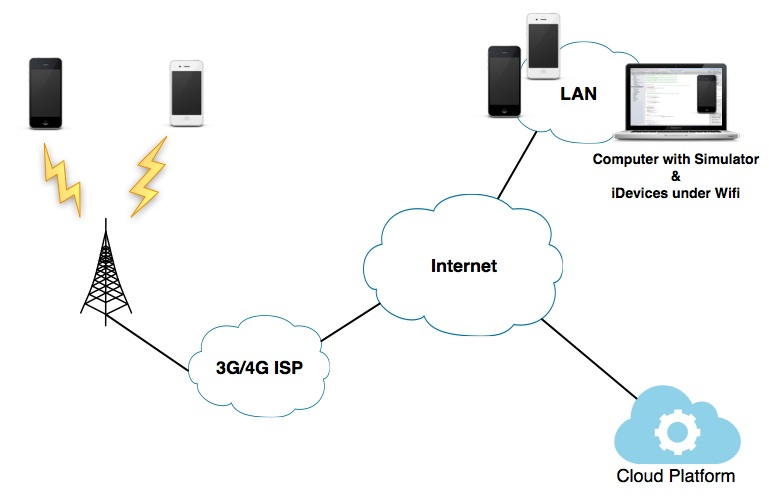
\includegraphics[width=0.8\textwidth]{./Images/test_env}
\caption{Test Environment}
\label{fig:test_env}
\end{figure}

Aliquam aliquet, est a ullamcorper condimentum, tellus nulla fringilla elit, a iaculis nulla turpis sed wisi. Fusce volutpat. Etiam sodales ante id nunc. Proin ornare dignissim lacus. Nunc porttitor nunc a sem. Sed sollicitudin velit eu magna. Aliquam erat volutpat. Vivamus egestas. Nunc tempor diam vehicula mauris. Nullam sapien eros, facilisis vel, eleifend non, auctor dapibus, pede \ref{tab:network_profiles} used in the tests. The Network Link Conditioner allows to force/simulate fluctuations in fixed network segments.

\begin{table}[htb]
\centering
\normalsize
    \caption{Network Link Conditioner Profiles}
    \label{tab:network_profiles}
{\footnotesize
    \begin{tabular}{ | c | c | c | c | }
    \hline 
    \textbf{Network Profile}	& \textbf{Bandwidth} & \textbf{Packets Droped} & \textbf{Delay}\\ \hline \hline
    Wifi  & 40 mbps  &  0\%  &   1 ms \\ \hline
    3G  & 780 kbps  &  0\%  &   100 ms \\ \hline 
    Edge  & 240 kbps  &  0\%  &   400 ms \\ \hline
    \end{tabular}
    }
\end{table}

Aliquam aliquet, est a ullamcorper condimentum, tellus nulla fringilla elit, a iaculis nulla turpis sed wisi. Fusce volutpat. Etiam sodales ante id nunc. Proin ornare dignissim lacus. Nunc porttitor nunc a sem. Sed sollicitudin velit eu magna. Aliquam erat volutpat. Vivamus ornare est non wisi. Proin vel quam. Vivamus egestas. Nunc tempor diam vehicula mauris. Nullam sapien eros, facilisis vel, eleifend non, auctor dapibus, pede.
% #############################################################################
\section{Proin ornare dignissim lacus}
Pellentesque habitant morbi tristique senectus et netus et malesuada fames ac turpis egestas. Vestibulum tortor quam, feugiat vitae, ultricies eget, tempor sit amet, ante. Donec eu libero sit amet quam egestas semper. Aenean ultricies mi vitae est. Mauris placerat eleifend leo. Quisque sit amet est et sapien ullamcorper pharetra. Vestibulum erat wisi, condimentum sed, commodo vitae, ornare sit amet, wisi. Aenean fermentum, elit eget tincidunt condimentum, eros ipsum rutrum orci, sagittis tempus lacus enim ac dui. Donec non enim in turpis pulvinar facilisis. Ut felis.

Et ``optimistic'' nulla dui purus, eleifend vel, consequat non, dictum porta, nulla. Duis ante mi, laoreet ut, commodo eleifend, cursus nec, lorem. Aenean eu est. Etiam imperdiet turpis. Praesent nec augue. Curabitur ligula quam, rutrum id, tempor sed, consequat ac, dui $G_j$, nec ligula et lorem consequat ullamcorper $p$ ut mauris eu mi mollis luctus $j$, porttitor ut, \ref{unchoke_gain}, uctus posuere justo:

\begin{description}
  \item[$N_j$] Is the number of times peer $j$ has been optimistically unchoked.
  \item[$n_j$] Among the $N_j$ unchokes, the number of times that peer $j$ responded with unchoke or supplied segments to peer $p$.
  \item[$C_{r[j]}$] The cooperation ratio of peer $j$. If peer $j$ never supplied peer $p$, the information of $C_{r[j]}$ may not be available.
  \item[$C_{r (max)}$] The maximum cooperation ratio of peer $p$’s neighbors, i.e., $C_{r (max)} = max(C_r)$.
\end{description}

\begin{equation}
\label{unchoke_gain}
 G_j =
  \begin{dcases}
    \frac{n_j C_{r[j]}}{N_j} &\quad \text{if } n_j > 0\\
    \frac{C_{r (max)}}{N_j + 1} &\quad \text{if } n_j = 0
  \end{dcases}
\end{equation}

Cursus $C_{r (max)}$ conubia nostra, per inceptos hymenaeos $j$ gadipiscing mollis massa $N_j = 0$, unc ut dui eget nulla venenatis aliquet $G_j = C_{r (max)}$.

Vestibulum accumsan eros nec magna. Vestibulum vitae dui. Vestibulum nec ligula et lorem consequat ullamcorper. Class aptent taciti sociosqu ad litora torquent per conubia nostra, per inceptos hymenaeos. Phasellus eget nisl ut elit porta ullamcorper. Maecenas tincidunt velit quis orci. Sed in dui. Nullam ut mauris eu mi mollis luctus. Class aptent taciti sociosqu ad litora torquent per conubia nostra, per inceptos hymenaeos. Sed cursus cursus velit. Sed a massa. 

Both \ref{fig:tx_layer_4,fig:tx_layer_5} Phasellus eget nisl ut elit porta ``perfect'' tincidunt. Class aptent taciti sociosqu ad litora torquent per conubia nostra.

\begin{figure}[h]
%\centering
       \subfigure[Adaptation System Test 4]{\label{fig:tx_layer_4}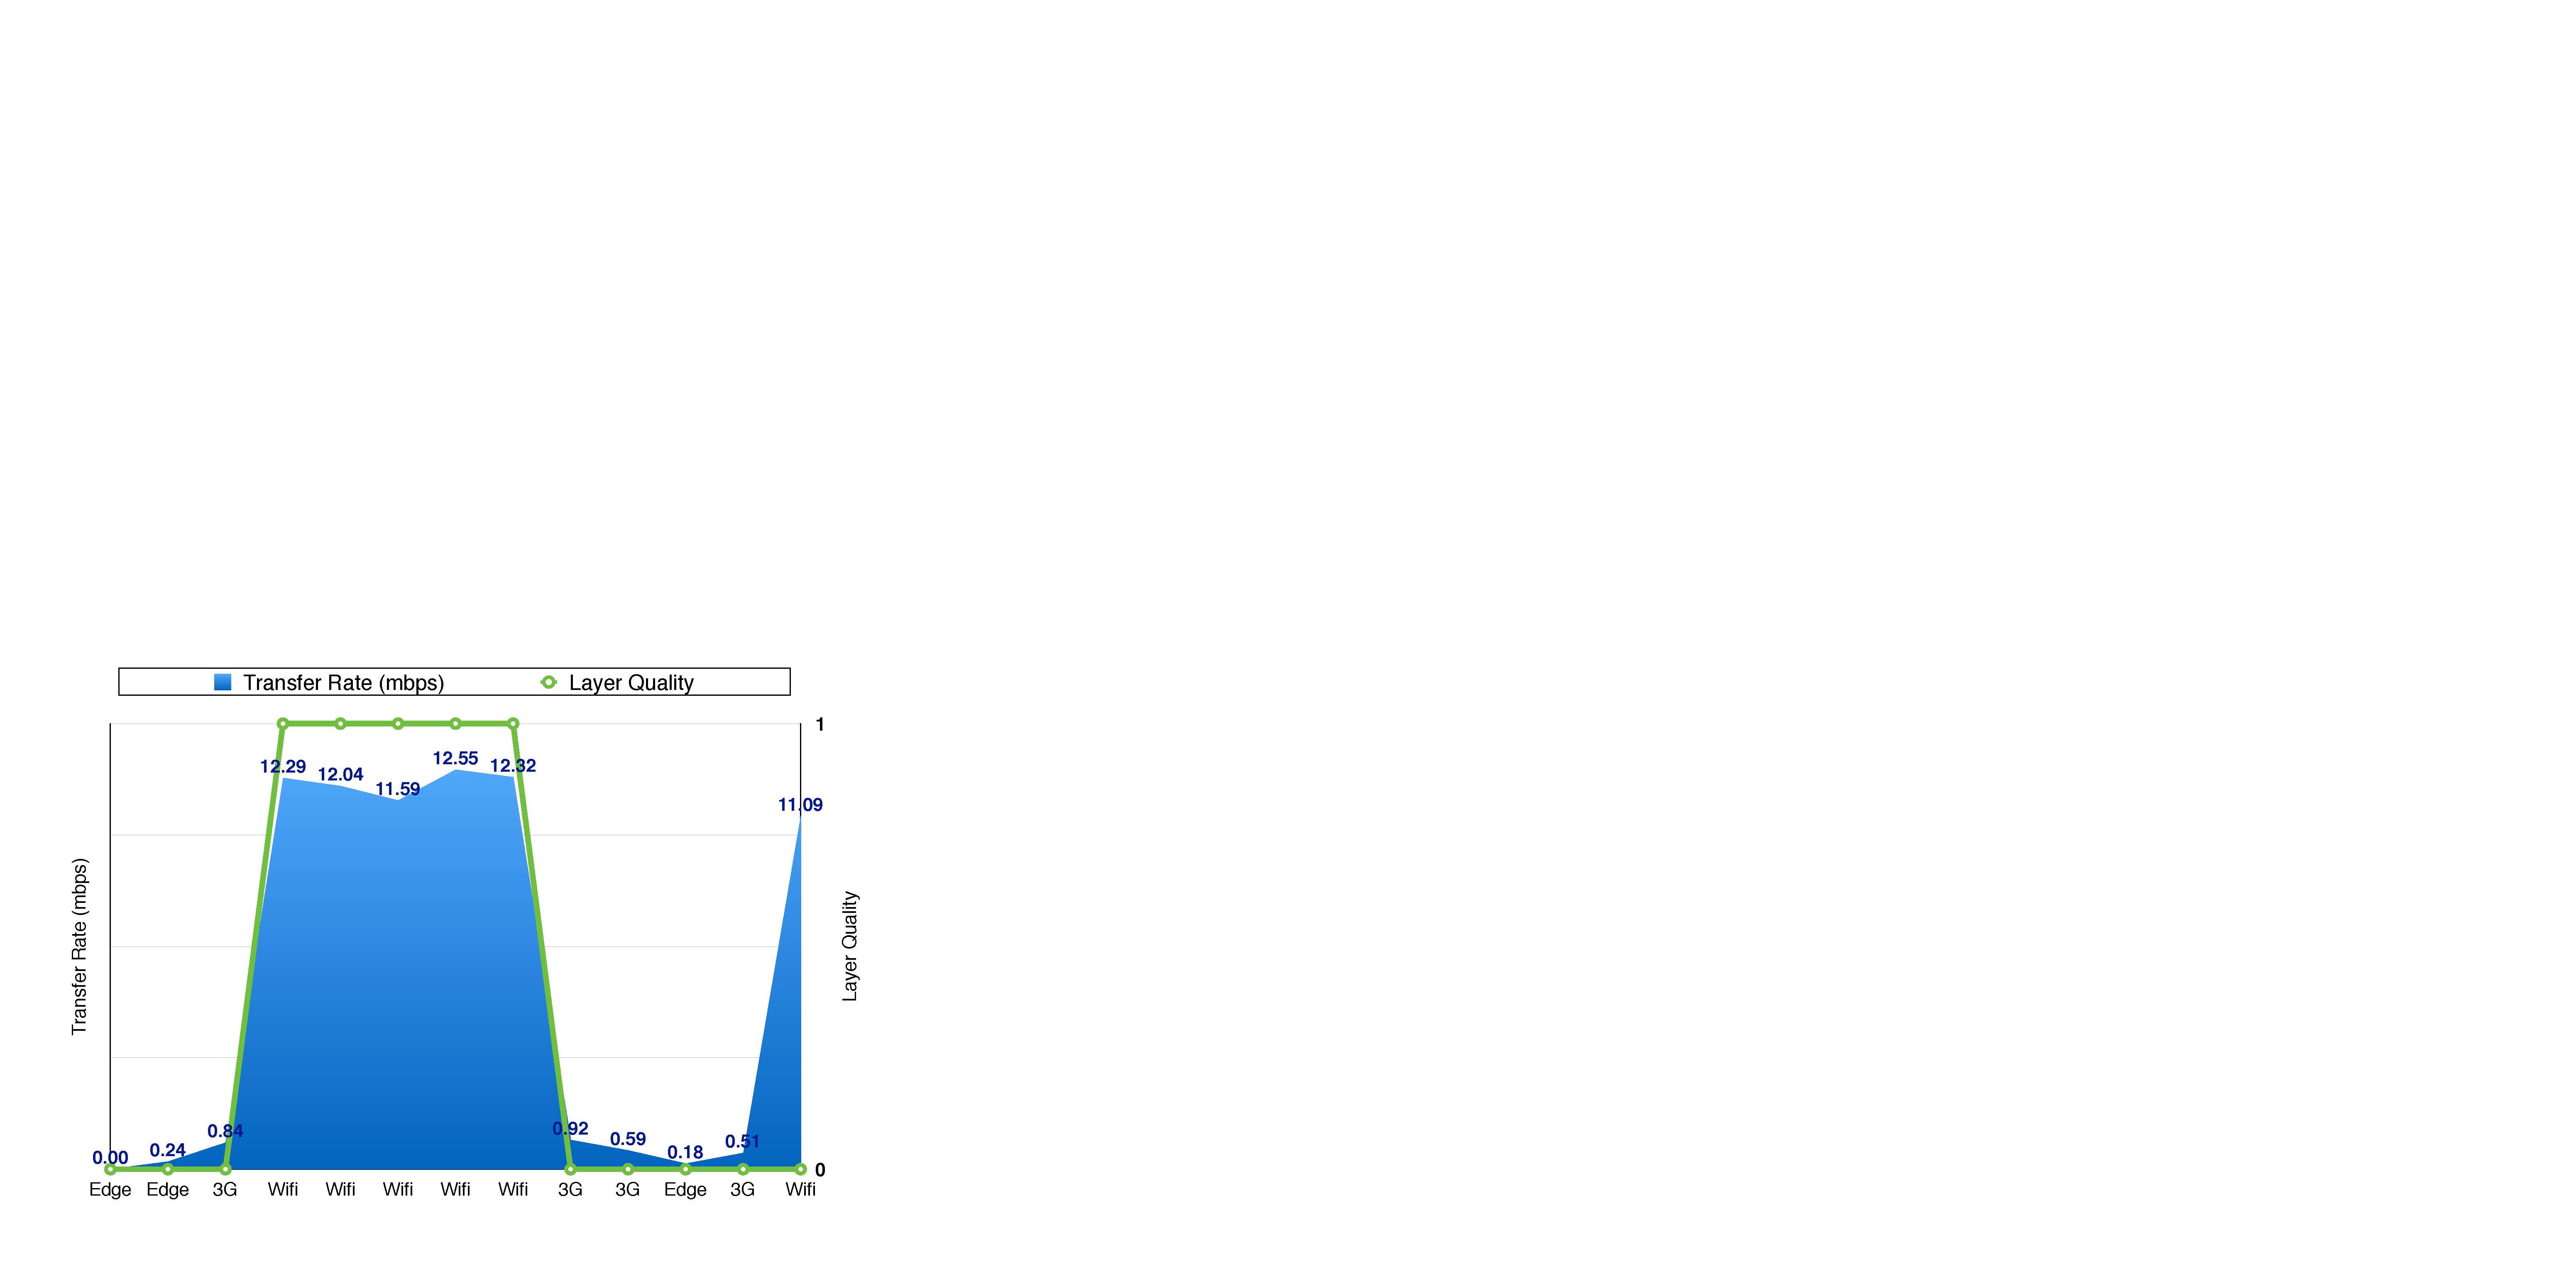
\includegraphics[width=0.5\textwidth]{./Images/tx_layer_4}}  
   %    \centering 
       \subfigure[Adaptation System Test 5]{\label{fig:tx_layer_5}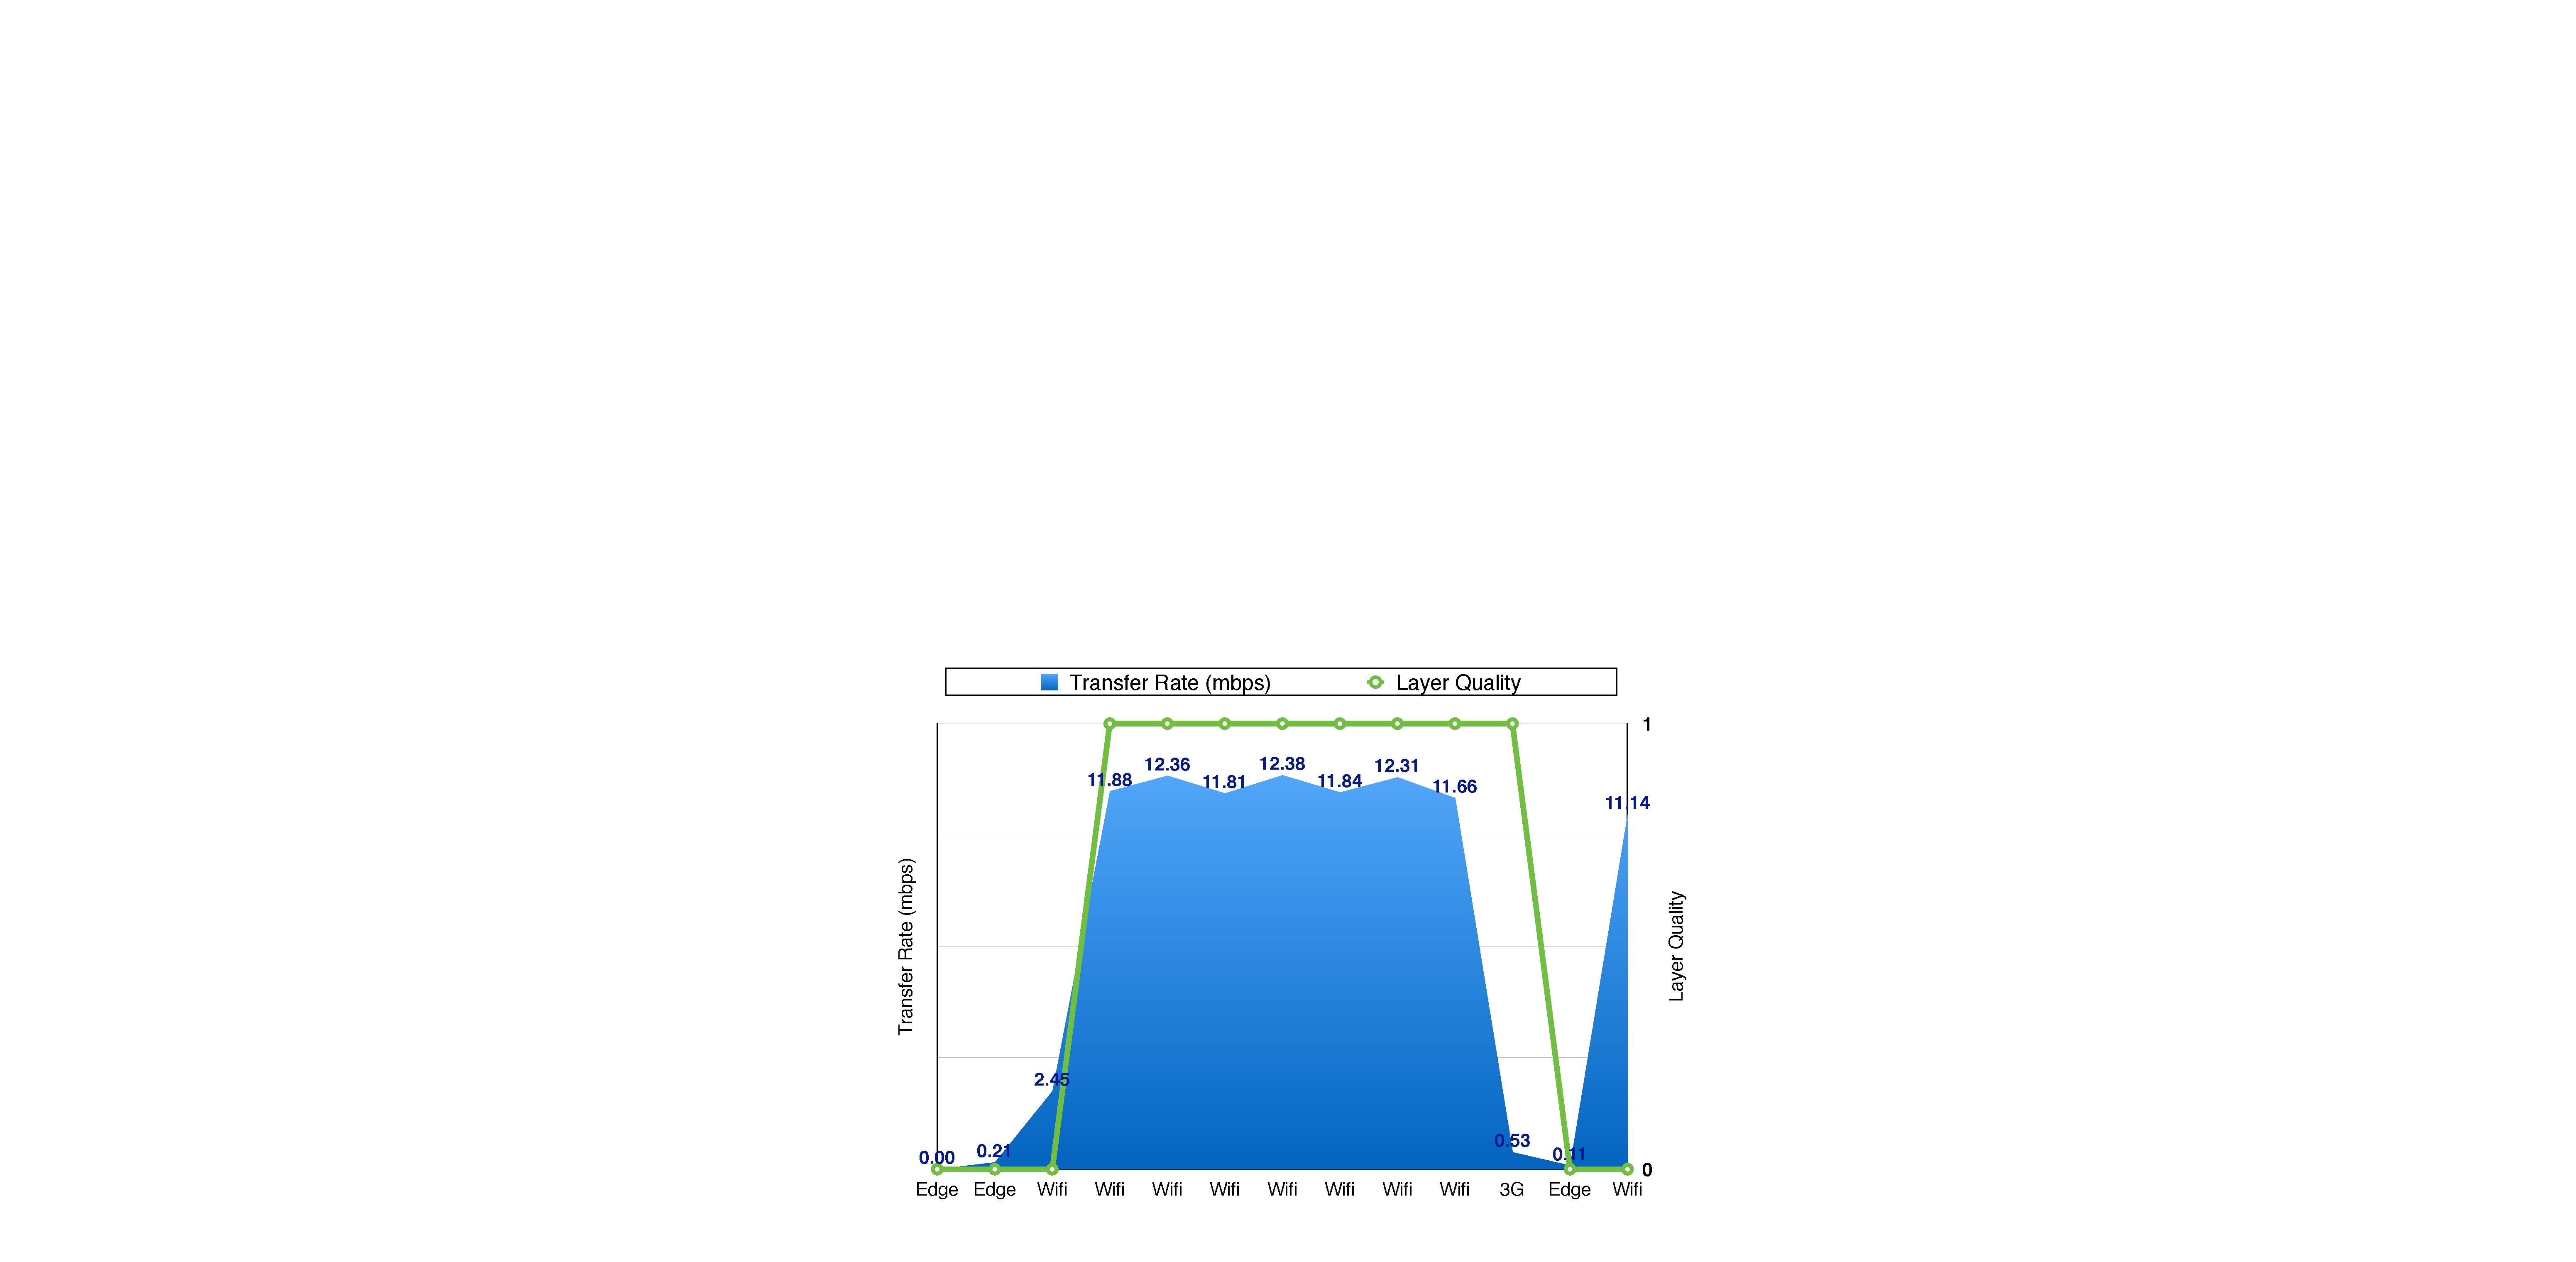
\includegraphics[width=0.5\textwidth]{./Images/tx_layer_5}}   
        \caption{Adaptation System Behavior Test}
        \label{fig:fig:adapt_behave_2}
\end{figure}

Cras sed ante. Phasellus in massa. Curabitur dolor eros, gravida et, hendrerit ac, cursus non, massa. Aliquam lorem. In hac habitasse platea dictumst. Cras eu mauris. Quisque lacus. Donec ipsum. Nullam vitae sem at nunc pharetra ultricies. Vivamus elit eros, ullamcorper a, adipiscing sit amet, porttitor ut, nibh. Maecenas adipiscing mollis massa. Nunc ut dui eget nulla venenatis aliquet. Sed luctus posuere justo. Cras vehicula varius turpis. Vivamus eros metus, tristique sit amet, molestie dignissim, malesuada et, urna.
% If Printing on DOUBLE SIDED pages, the second page should be white.
% Otherwise, comment the following command:
\cleardoublepage
%
%Chapter 6
% #############################################################################
% This is Chapter 6
% !TEX root = ../main.tex
% #############################################################################
% Change the Name of the Chapter i the following line
\chapter{Conclusion}
\chaptoc
\label{chap:conclusion}
\bigskip

 
% #############################################################################
\section{Conclusions}

% #############################################################################
\section{System Limitations and Future Work}
% If Printing on DOUBLE SIDED pages, the second page should be white.
% Otherwise, comment the following command:
%\cleardoublepage
%
% -----------------------------------------------------------------------------
% BIBLIOGRAPHY
% Add the Bibliography to the PDF table of contents (not the document table of contents)
%\pdfbookmark[0]{Bibliography}{bib}
\addcontentsline{toc}{chapter}{Bibliography}
% The bibliography style sheet
% Chose your preferences on the format of the entries and the Labels:
% IEEEtran: Used in general (recommended for IST Thesis)
%           Entries are labelled and sorted by appearance in the document
%           Labels are Numeric inside square brackets
\bibliographystyle{IEEEtran}
%
% Apalike:  Entries formatted alphabetically, last name first, with identation
%           Labels with Autor's Name and Year inside square brackets
%\bibliographystyle{apalike}
%
% Alpha:    Entries formatted with Autor's Name and Year, hanging identation
%           Labels with Autor's abbr. Names and Year inside square brackets
%\bibliographystyle{alpha}
%
% Acm:     Entries formatted with Autor's Name (small Caps), hanging identation
%          Labels are Numeric inside square brackets
%\bibliographystyle{acm}
% The following command resets the 'emphasis' style for bibliography entries
\normalem
% Name of your BiBTeX file
\bibliography{./Bibliography} % Put here your own filename
%
% The following command modifies the 'emphasis' style for bibliography entries
\ULforem
% If Printing on DOUBLE SIDED pages, the second page should be white.
% Otherwise, comment the following command:
%\cleardoublepage
%

% If Printing on DOUBLE SIDED pages, the second page should be white.
%\clearpage
% Otherwise, comment the following command:
%\cleardoublepage
% -----------------------------------------------------------------------------
% HERE GO THE APPENDIXES IF REQUIRED
% If not required just comment the blocks
\appendix
%% First Appendix
%\pdfbookmark[1]{Appendix A}{appendix}
% #############################################################################
% This is Appendix A
% !TEX root = ../main.tex
% #############################################################################
\chapter{Code of Project}
\label{chapter:appendixA}



% Nulla dui purus, eleifend vel, consequat non, dictum porta, nulla. Duis ante mi, laoreet ut, commodo eleifend, cursus nec, lorem. Aenean eu est. Etiam imperdiet turpis. Praesent nec augue. Curabitur ligula quam, rutrum id, tempor sed, consequat ac, dui. Vestibulum accumsan eros nec magna. Vestibulum vitae dui. Vestibulum nec ligula et lorem consequat ullamcorper. 

% \begin{lstlisting}[frame=lines,style=XML,caption={Example of a XML file.},label=xmlEx]
% <?xml version="1.0" encoding="UTF-8"?>
% <StreamInfo version="2.0">
%     <Clip duration="PT01M0.00S">
%         <BaseURL>videos/</BaseURL>
%         <Description>svc_1</Description>
%         <Representation mimeType="video/SVC" codecs="svc" frameRate="30.00" bandwidth="401.90"
%             width="176" height="144" id="L0">
%             <BaseURL>svc_1/</BaseURL>
%             <SegmentInfo from="0" to="11" duration="PT5.00S">
%                 <BaseURL>svc_1-L0-</BaseURL>
%             </SegmentInfo>
%         </Representation>
%         <Representation mimeType="video/SVC" codecs="svc" frameRate="30.00" bandwidth="1322.60"
%             width="352" height="288" id="L1">
%             <BaseURL>svc_1/</BaseURL>
%             <SegmentInfo from="0" to="11" duration="PT5.00S">
%                 <BaseURL>svc_1-L1-</BaseURL>
%             </SegmentInfo>
%         </Representation>
%     </Clip>
% </StreamInfo>
% \end{lstlisting}

% Etiam imperdiet turpis. Praesent nec augue. Curabitur ligula quam, rutrum id, tempor sed, consequat ac, dui. Maecenas tincidunt velit quis orci. Sed in dui. Nullam ut mauris eu mi mollis luctus. Class aptent taciti sociosqu ad litora torquent per conubia nostra, per inceptos hymenaeos. Sed cursus cursus velit. Sed a massa. Duis dignissim euismod quam.


% Class aptent taciti sociosqu ad litora torquent per conubia nostra, per inceptos hymenaeos. Phasellus eget nisl ut elit porta ullamcorper. Maecenas tincidunt velit quis orci. Sed in dui. Nullam ut mauris eu mi mollis luctus. Class aptent taciti sociosqu ad litora torquent per conubia nostra, per inceptos hymenaeos.

% This inline MATLAB code \mcode{for i=1:3, disp('cool'); end;} uses the \verb|\mcode{}| command.\footnote{MATLAB Works also in footnotes: \mcodefn{for i=1:3, disp('cool'); end;}}

% Nullam ut mauris eu mi mollis luctus. Class aptent taciti sociosqu ad litora torquent per conubia nostra, per inceptos hymenaeos. Sed cursus cursus velit. Sed a massa. Duis dignissim euismod quam. Nullam euismod metus ut orci.

% \begin{lstlisting}[language=matlabfloz,caption={\mcode{Matlab Function}}]
% for i = 1:3
% 	if i >= 5 && a ~= b       % literate programming replacement
% 		disp('cool');         % comment with some §\mcommentfont\LaTeX in it: $\mcommentfont\pi x^2$§
% 	end
% 	[:,ind] = max(vec);
% 	x_last = x(1,end) - 1;
% 	v(end);
% 	ylabel('Voltage (µV)');
% end
% \end{lstlisting}

% Nullam ut mauris eu mi mollis luctus. Class aptent taciti sociosqu ad litora torquent per conubia nostra, per inceptos hymenaeos. Sed cursus cursus velit. Sed a massa. Duis dignissim euismod quam. Nullam euismod metus ut orci.

% \lstinputlisting[
% 	label=lst:matlab_code,
% 	caption={\mcode{function.m}},
% 	breaklines=true
% 	]{./tables_and_code/function.m}

% Class aptent taciti sociosqu ad litora torquent per conubia nostra, per inceptos hymenaeos. Phasellus eget nisl ut elit porta ullamcorper. Maecenas tincidunt velit quis orci. Sed in dui. Nullam ut mauris eu mi mollis luctus. Class aptent taciti sociosqu ad litora torquent per conubia nostra, per inceptos hymenaeos. Sed cursus cursus velit. Sed a massa. Duis dignissim euismod quam. Nullam euismod metus ut orci. Vestibulum erat libero, scelerisque et, porttitor et, varius a, leo.

% \begin{lstlisting}[style=htmlcssjs,caption={HTML with CSS Code}]
% <!DOCTYPE html>
% <html>
%   <head>
%     <title>Listings Style Test</title>
%     <meta charset="UTF-8">
%     <style>
%       /* CSS Test */
%       * {
%         padding: 0;
%         border: 0;
%         margin: 0;
%       }
%     </style>
%     <link rel="stylesheet" href="css/style.css" />
%   </head>
%   <header> hey </header>
%   <article> this is a article </article>
%   <body>
%     <!-- Paragraphs are fine -->
%     <div id="box">			
% 			<p>
% 			  Hello World
% 			</p>
%       <p>Hello World</p>
%       <p id="test">Hello World</p>
% 			<p></p>
%     </div>
%     <div>Test</div>
%     <!-- HTML script is not consistent -->
%     <script src="js/benchmark.js"></script>
%     <script>
%       function createSquare(x, y) {
%         // This is a comment.
%         var square = document.createElement('div');
%         square.style.width = square.style.height = '50px';
%         square.style.backgroundColor = 'blue';
        
%         /*
%          * This is another comment.
%          */
%         square.style.position = 'absolute';
%         square.style.left = x + 'px'; 
%         square.style.top = y + 'px';
        
%         var body = document.getElementsByTagName('body')[0];
%         body.appendChild(square);
%       };
      
%       // Please take a look at +=
%       window.addEventListener('mousedown', function(event) {
%         // German umlaut test: Berührungspunkt ermitteln
%         var x = event.touches[0].pageX;
%         var y = event.touches[0].pageY;
%         var lookAtThis += 1;
%       });
%     </script>
%   </body>
% </html>
% \end{lstlisting}

% Nulla dui purus, eleifend vel, consequat non, dictum porta, nulla. Duis ante mi, laoreet ut, commodo eleifend, cursus nec, lorem. Aenean eu est. Etiam imperdiet turpis. Praesent nec augue. Curabitur ligula quam, rutrum id, tempor sed, consequat ac, dui. Vestibulum accumsan eros nec magna. Vestibulum vitae dui. Vestibulum nec ligula et lorem consequat ullamcorper.

% \begin{lstlisting}[style=htmlcssjs,caption={HTML CSS Javascript Code}]

% @media only screen and (min-width: 768px) and (max-width: 991px) {
	
% 	#main {
% 		width: 712px;
% 		padding: 100px 28px 120px;
% 	}
	
% 	/* .mono {
% 		font-size: 90%;
% 	} */
	
% 	.cssbtn a {
% 		margin-top: 10px;
% 		margin-bottom: 10px;
% 		width: 60px;  
% 		height: 60px;   
% 		font-size: 28px;
% 		line-height: 62px;
% 	}
% \end{lstlisting}

% Nulla dui purus, eleifend vel, consequat non, dictum porta, nulla. Duis ante mi, laoreet ut, commodo eleifend, cursus nec, lorem. Aenean eu est. Etiam imperdiet turpis. Praesent nec augue. Curabitur ligula quam, rutrum id, tempor sed, consequat ac, dui. Vestibulum accumsan eros nec magna. Vestibulum vitae dui. Vestibulum nec ligula et lorem consequat ullamcorper.

% \begin{lstlisting} [style=py,caption={PYTHON Code}]
% class TelgramRequestHandler(object):
%     def handle(self):
%         addr = self.client_address[0]         # Client IP-adress
%         telgram = self.request.recv(1024)     # Recieve telgram
%         print "From: %s, Received: %s" % (addr, telgram)
%         return
% \end{lstlisting}
%% If Printing on DOUBLE SIDED pages, the second page should be white.
%% Otherwise, comment the following command:
\cleardoublepage
%% Second Appendix
%\pdfbookmark[1]{Appendix B}{appendix}
% #############################################################################
% This is Appendix B
% !TEX root = ../main.tex
% #############################################################################
\chapter{A Large Table}
\label{chapter:appendixB}

%% If Printing on DOUBLE SIDED pages, the second page should be white.
%% Otherwise, comment the following command:

% -----------------------------------------------------------------------------
% And this is THE END of the IST Thesis Document
\end{document}